\documentclass[supercite]{Experimental_Report}

\title{~~~~~~数据结构实验~~~~~~}
\author{王李超}
%\coauthor{张三、李四}
\school{计算机科学与技术学院}
\classnum{CS启明2401}
\stunum{U202414887}
%\costunum{U202115631、U202115631}
\instructor{王雄} % 该系列实验报告模板有华科大计院教师陈加忠制作
\date{2025年6月1日}

\usepackage{algorithm, multirow}
\usepackage{algpseudocode}
\usepackage{amsmath}
\usepackage{amsthm}
\usepackage{framed}
\usepackage{mathtools}
\usepackage{fix-cm}
\usepackage{fontspec}
\usepackage{subcaption}
\usepackage{xltxtra} %提供了针对XeTeX的改进并且加入了XeTeX的LOGO, 自动调用xunicode宏包(提供Unicode字符宏)
\usepackage{bm}
\usepackage{tabularx}
\usepackage{ltablex}
\usepackage{tikz}
\usepackage{tikzscale}
\usepackage{pgfplots}
\usepackage{caption}
%\usepackage{enumerate}
\usepackage{listings} % 引入 listings 宏包
\usepackage{xcolor}   % 用于自定义代码颜色
% 自定义代码样式
\lstset{
  language=C++,                % 设置语言为 C++
  basicstyle=\ttfamily\small,  % 设置代码字体和大小
  keywordstyle=\color{blue},   % 关键字颜色
  commentstyle=\color{green},  % 注释颜色
  stringstyle=\color{red},     % 字符串颜色
  numbers=left,                % 显示行号
  numberstyle=\tiny\color{gray}, % 行号样式
  stepnumber=1,                % 行号递增步长
  breaklines=true,             % 自动换行
  frame=single,                % 添加边框
  tabsize=4,                    % Tab 宽度
  lineskip=2pt             % 行间距
}

\pgfplotsset{compat=1.16}

\newcommand{\cfig}[3]{
  \begin{figure}[htb]
    \centering
    \includegraphics[width=#2\textwidth]{images/#1.tikz}
    \caption{#3}
    \label{fig:#1}
  \end{figure}
}

\newcommand{\sfig}[3]{
  \begin{subfigure}[b]{#2\textwidth}
    \includegraphics[width=\textwidth]{images/#1.tikz}
    \caption{#3}
    \label{fig:#1}
  \end{subfigure}
}

\newcommand{\xfig}[3]{
  \begin{figure}[htb]
    \centering
    #3
    \caption{#2}
    \label{fig:#1}
  \end{figure}
}

\newcommand{\rfig}[1]{\autoref{fig:#1}}
\newcommand{\ralg}[1]{\autoref{alg:#1}}
\newcommand{\rthm}[1]{\autoref{thm:#1}}
\newcommand{\rlem}[1]{\autoref{lem:#1}}
\newcommand{\reqn}[1]{\autoref{eqn:#1}}
\newcommand{\rtbl}[1]{\autoref{tbl:#1}}

\algnewcommand\Null{\textsc{null }}
\algnewcommand\algorithmicinput{\textbf{Input:}}
\algnewcommand\Input{\item[\algorithmicinput]}
\algnewcommand\algorithmicoutput{\textbf{Output:}}
\algnewcommand\Output{\item[\algorithmicoutput]}
\algnewcommand\algorithmicbreak{\textbf{break}}
\algnewcommand\Break{\algorithmicbreak}
\algnewcommand\algorithmiccontinue{\textbf{continue}}
\algnewcommand\Continue{\algorithmiccontinue}
\algnewcommand{\LeftCom}[1]{\State $\triangleright$ #1}

\newtheorem{thm}{定理}[section]
\newtheorem{lem}{引理}[section]

\colorlet{shadecolor}{black!15}

\theoremstyle{definition}
\newtheorem{alg}{算法}[section]

\def\thmautorefname~#1\null{定理~#1~\null}
\def\lemautorefname~#1\null{引理~#1~\null}
\def\algautorefname~#1\null{算法~#1~\null}

\begin{document}

\maketitle

\clearpage

\pagenumbering{Roman}

\tableofcontents[level=2]

\clearpage

\pagenumbering{arabic}

\section{基于顺序存储结构的线性表实现}



\subsection{问题描述}

\subsubsection{实验目的}
通过实验达到:(1)加深对线性表的概念、基本运算的理解;(2)熟练掌握线性表的逻辑结构与物理结构的关系;(3)物理结构采用顺序表,熟练掌握顺序表基本运算的实现。

\subsubsection{具体问题}

在设计线性表时,需要解决以下具体问题:
\begin{itemize}
	\item \textbf{存储结构的选择:} 选择顺序存储结构还是链式存储结构,需权衡存储效率和操作效率。
	\item \textbf{容量的动态扩展:} 当线性表存储空间不足时,如何动态扩展存储容量以容纳更多元素。
	\item \textbf{基本操作的实现:} 包括插入、删除、查找、更新等操作的具体实现及其时间复杂度优化。
	\item \textbf{边界条件处理:} 如何处理空表、满表以及非法操作(如越界访问)等特殊情况。
	\item \textbf{数据类型的通用性:} 设计线性表时,如何支持存储多种数据类型(如整数、浮点数、字符串等)。
	\item \textbf{内存管理:} 如何高效管理内存,避免内存泄漏或冗余分配。
	\item \textbf{算法效率:} 针对不同操作需求,优化算法以提高线性表的整体性能。
\end{itemize}


\subsection{系统设计}

整体系统结构设计方面,本系统采用模块化设计思想,将顺序表的各项操作功能(如初始化、插入、删除、查找、遍历、排序、文件读写等)分别封装为独立的函数,并通过主程序 main01.cpp 提供统一的菜单式交互界面,方便用户进行各类操作。系统支持多顺序表管理,用户可新建、删除、切换和重命名多个顺序表,提升了系统的灵活性和扩展性。各功能模块之间通过头文件(如 def.h、func.h)进行数据类型和函数声明的解耦,便于维护和升级。

数据结构设计方面,核心采用顺序存储结构实现线性表。定义了 SqList 结构体,包含元素指针和当前长度等信息,实现了线性表的基本操作。为支持多顺序表管理,设计了 LISTS 结构体,内部维护一个顺序表数组,每个元素包含一个 SqList 及其名称。元素类型 ElemType 可根据实际需求灵活定义。通过结构体嵌套和指针管理,系统实现了对多个线性表的统一管理和操作,保证了数据的有序性和高效性。整体设计兼顾了功能完整性、易用性和可扩展性。

\subsection{系统实现}

主要说明各个主要函数的实现思想,复杂函数可辅助流程图进行说明,函数和系统实现的源代码放在附录中。

\subsubsection{主要函数实现思想}

\begin{itemize}
    \item \textbf{InitList}:判断线性表是否已存在,若不存在则分配初始空间,初始化长度和容量。
    \item \textbf{DestroyList}:释放线性表空间,并将指针和长度等信息重置,防止内存泄漏。
    \item \textbf{ClearList}:不释放空间,仅将长度归零,实现逻辑清空。
    \item \textbf{ListEmpty}:判断线性表是否存在及是否为空,返回相应状态。
    \item \textbf{ListLength}:返回线性表当前长度,若不存在则返回异常。
    \item \textbf{GetElem}:获取指定位置元素,先判断合法性和存在性。
    \item \textbf{LocateElem}:顺序查找指定元素,返回其逻辑序号,未找到返回0。
    \item \textbf{PriorElem/NextElem}:查找指定元素的前驱或后继,遍历查找并返回相邻元素。
    \item \textbf{ListInsert}:判断插入位置合法性,必要时扩容,移动元素后插入新元素。
    \item \textbf{ListDelete}:判断删除位置合法性,保存被删元素,移动后续元素覆盖。
    \item \textbf{ListTraverse}:顺序输出所有元素,便于调试和展示。
    \item \textbf{MaxSubArray}:实现最大连续子数组和的求解,采用动态规划思想。
    \item \textbf{SubArrayNum}:统计和为指定值的子数组个数,双重循环遍历所有子区间。
    \item \textbf{sortList}:采用冒泡排序对顺序表元素排序。
    \item \textbf{saveListToFile/loadListFromFile}:实现顺序表的文件保存与加载,便于数据持久化。
    \item \textbf{manageMultipleLists}:输出当前所有顺序表及其名称,实现多表管理。
    \item \textbf{AddList/RemoveList/LocateList}:实现多顺序表的添加、删除和查找,支持名称唯一性和内存管理。
\end{itemize}

\subsubsection{部分函数实现方法}

以下选取几个实现较为复杂或具有代表性的函数,简要说明其实现思路,并给出伪代码辅助理解。

\paragraph{1. ListInsert(顺序表插入)}
该函数需判断插入位置是否合法,若空间不足则动态扩容,然后将插入位置及其后的元素依次后移,最后插入新元素。

\begin{shaded*}
\begin{alg}{ListInsert(顺序表插入)}
    \label{alg:ListInsert}
    \begin{algorithmic}
        \Input 顺序表 $L$,插入位置 $i$,元素 $e$
        \Output 插入是否成功
        \If{$L$ 不存在}
            \State \Return INFEASIBLE
        \EndIf
        \State 检查内存分配是否成功
        \For{$j = L.length$ \textbf{downto} $i$}
            \State $L.elem[j] \gets L.elem[j-1]$
        \EndFor
        \State 将元素插入到位置 $i$:$L.elem[i-1] \gets e$
        \State \Return OK
    \end{algorithmic}
\end{alg}
\end{shaded*}

\paragraph{2. ListDelete(顺序表删除)}
首先判断删除位置是否合法,保存被删元素,然后将其后的元素依次前移,最后长度减一。

\begin{shaded*}
\begin{alg}{ListDelete(顺序表删除)}
    \label{alg:ListDelete}
    \begin{algorithmic}
        \Input 顺序表 $L$,删除位置 $i$
        \Output 被删除元素 $e$,删除是否成功
        \If{$L$ 不存在}
            \State \Return INFEASIBLE
        \EndIf
        \State 检查删除位置合法性
        \State $e \gets L.elem[i-1]$
        \For{$j = i$ \textbf{to} $L.length-1$}
            \State $L.elem[j-1] \gets L.elem[j]$
        \EndFor
        \State 顺序表长度减一
        \State \Return OK
    \end{algorithmic}
\end{alg}
\end{shaded*}

\paragraph{3. MaxSubArray(最大连续子数组和)}
采用动态规划思想,遍历数组,记录当前子数组和与最大值。

\begin{shaded*}
\begin{alg}{MaxSubArray(最大连续子数组和)}
    \label{alg:MaxSubArray}
    \begin{algorithmic}
        \Input 顺序表 $L$
        \Output 最大连续子数组和 $maxSum$
        \State $maxSum \gets L.elem[0]$
        \State $currentSum \gets 0$
        \For{$i = 0$ \textbf{to} $L.length-1$}
            \If{$currentSum > 0$}
                \State $currentSum \gets currentSum + L.elem[i]$
            \Else
                \State $currentSum \gets L.elem[i]$
            \EndIf
            \If{$currentSum > maxSum$}
                \State $maxSum \gets currentSum$
            \EndIf
        \EndFor
        \State \Return $maxSum$
    \end{algorithmic}
\end{alg}
\end{shaded*}

\paragraph{4. AddList(多顺序表添加)}
支持批量添加,需判断名称唯一性,动态分配空间,并循环插入元素直到输入0结束。

\begin{shaded*}
\begin{alg}{AddList(多顺序表添加)}
    \label{alg:AddList}
    \begin{algorithmic}
        \Input 多顺序表 $Lists$,新表名称 $ListName$
        \Output 添加是否成功
        \For{每个待添加顺序表}
            \While{名称重复}
                \State 提示重新输入 $ListName$
            \EndWhile
            \If{顺序表数量已达上限}
                \State \Return ERROR
            \EndIf
            \State 分配新表空间,初始化
            \While{输入元素 $e \neq 0$}
                \State 插入 $e$ 到新表
            \EndWhile
            \State 添加成功
        \EndFor
        \State \Return OK
    \end{algorithmic}
\end{alg}
\end{shaded*}

\subsection{系统测试}

\begin{figure}[htb]
	\begin{center}
		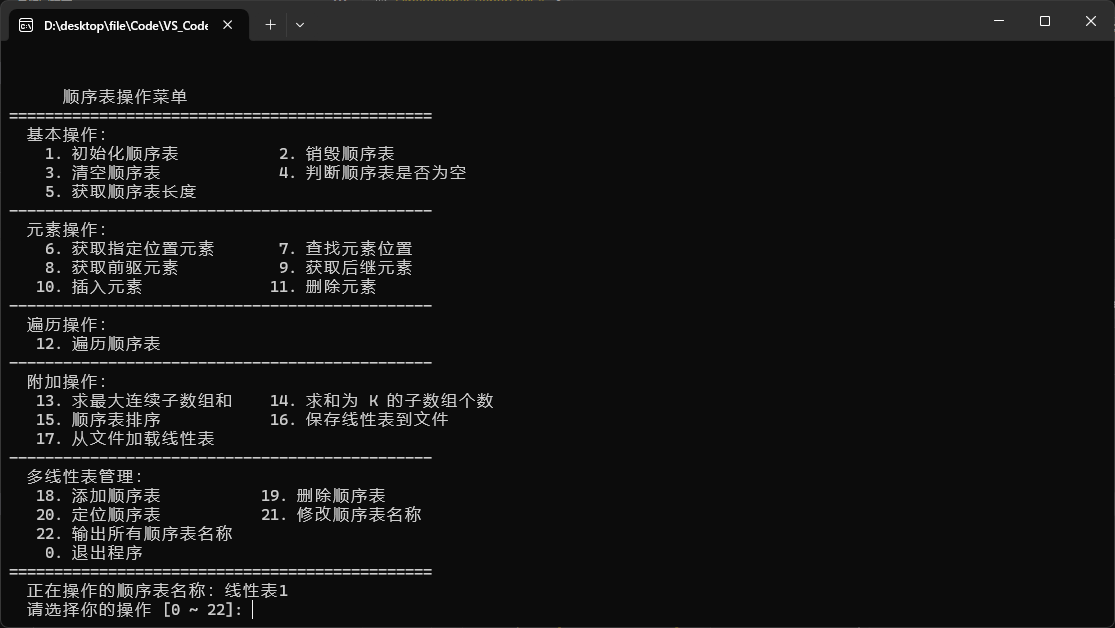
\includegraphics[scale=0.30]{images/1-1.jpg}
		\caption{线性表操作界面}
		\label{fig1-1}
	\end{center}
\end{figure}

主要说明针对各个函数正常和异常的测试用例及测试结果。测试用例设计时,考虑了正常情况、边界条件(如\ref{table:seqlist-test}中多次创建、删除线性表,查询边界处元素)和异常情况等多种场景,确保系统的健壮性和稳定性。以下是部分测试用例及其结果:

\newpage

\subsubsection{基础功能测试}
    \begin{center}
        \setlength{\tabcolsep}{2.0mm}
        \captionof{table}{线性表主要功能测试用例及结果}
        \label{table:seqlist-test}
        \begin{tabularx}{\textwidth}{|X|X|X|}
            \hline
            测试功能及序号 & 输入 & 输出 \\\hline
            1. 构造空线性表 & \textbackslash & 线性表创建成功! \\\hline
            1. 构造空线性表 & \textbackslash & 线性表创建失败! \\\hline
            10. 插入元素(3次) & 4 1;6 2;8 3 & 插入成功!(3次) \\\hline
            4. 判空线性表 & \textbackslash & 线性表不是空表! \\\hline
            5. 求表长 & \textbackslash & 线性表的长度为:3 \\\hline
            6. 获取元素 & 2 & 线性表的第2个元素为:6 \\\hline
            7. 定位元素 & 8 & 线性表中元素8的序号为:3 \\\hline
            8. 获取前驱 & 4 & 线性表中元素4的前驱元素查找失败! \\\hline
            8. 获取前驱 & 6 & 线性表中元素6的前驱元素为:4 \\\hline
            9. 获取后继 & 8 & 线性表中元素8的后继元素查找失败! \\\hline
            9. 获取后继 & 4 & 线性表中元素4的后继元素为:6 \\\hline
            12. 遍历线性表 & \textbackslash & 4 6 8 \\\hline
            16. 文件保存/17. 文件读取 & \textbackslash & 保存成功!/载入成功! \\\hline
            11. 删除元素 & 2 & 线性表中元素6删除成功! \\\hline
            3. 清空线性表 & \textbackslash & 线性表清空成功! \\\hline
            2. 销毁线性表 & \textbackslash & 线性表销毁成功! \\\hline
            2. 销毁线性表 & \textbackslash & 线性表销毁失败! \\\hline
            0. 退出系统 & \textbackslash & 欢迎再次使用本系统! \\\hline
        \end{tabularx}
    \end{center}

\begin{figure}[htb]
	\begin{center}
		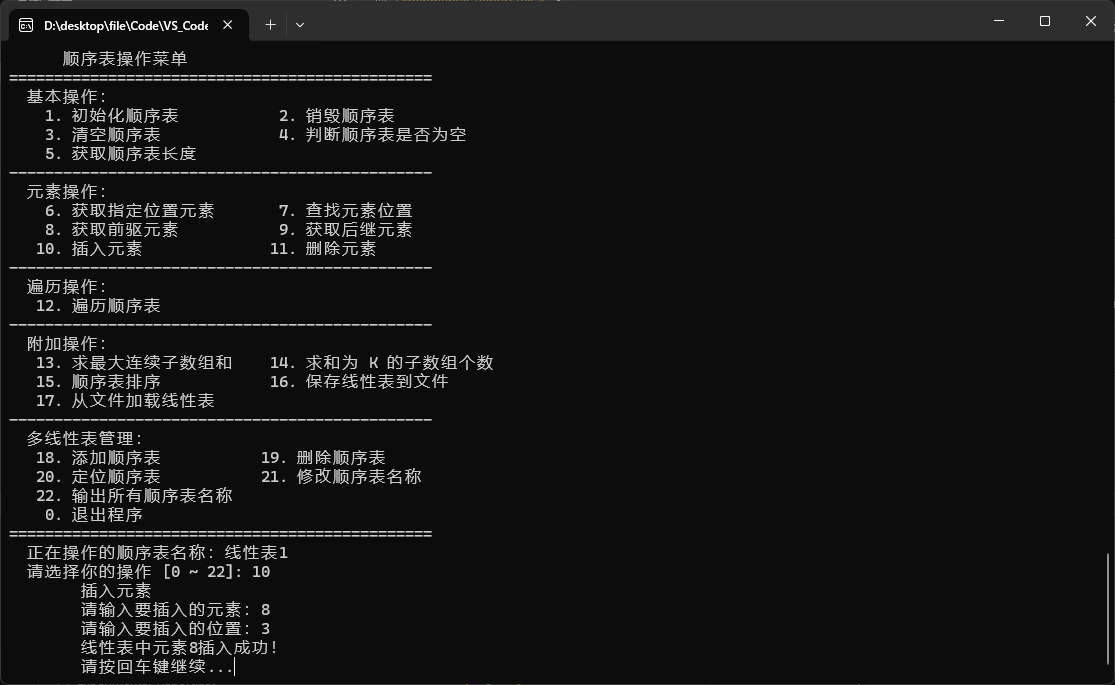
\includegraphics[scale=0.30]{images/1-2.jpg}
		\caption{基础功能测试截图}
		\label{fig1-2}
	\end{center}
\end{figure}

\subsubsection{附加功能测试}

    \begin{center}
        \setlength{\tabcolsep}{2.0mm}
        \captionof{table}{测试时初始状态}
        \label{table:start-status}
        \begin{tabularx}{\textwidth}{|X|X|}
            \hline
            表名称 & 数据 \\\hline
            a & 无  \\\hline
            b & 20 1 2 -4 10 -19 2 2 50  \\\hline
        \end{tabularx}

        \setlength{\tabcolsep}{2.0mm}
        \captionof{table}{线性表附加功能测试用例及结果}
        \label{table:more-seqlist-test}
        \begin{tabularx}{\textwidth}{|X|X|X|}
            \hline
            测试功能及序号 & 输入 & 输出 \\\hline
            13. 最大连续子数组和 & b & 最大连续子数组和为:55 \\\hline
            14. 和为指定值的子数组个数 & 1 2 -3 4 -5 6 7 -8 9 10 & 和为指定值的子数组个数为:0 \\\hline
            15. 顺序表排序 & b & 排序成功! \\\hline
            12. 遍历线性表 & \textbackslash & 20 1 2 -4 10 -19 2 2 50 \\\hline
            16. 文件保存 & \textbackslash & 保存成功! \\\hline
            3. 清空线性表 & \textbackslash & 线性表清空成功! \\\hline
            17. 文件读取 & \textbackslash & 载入成功! \\\hline
            12. 遍历线性表 & \textbackslash & 20 1 2 -4 10 -19 2 2 50 \\\hline
            22. 输出所有顺序表名称 & \textbackslash & 线性表名称:a b \\\hline
        \end{tabularx}
    \end{center}

\begin{figure}[htb]
	\begin{center}
		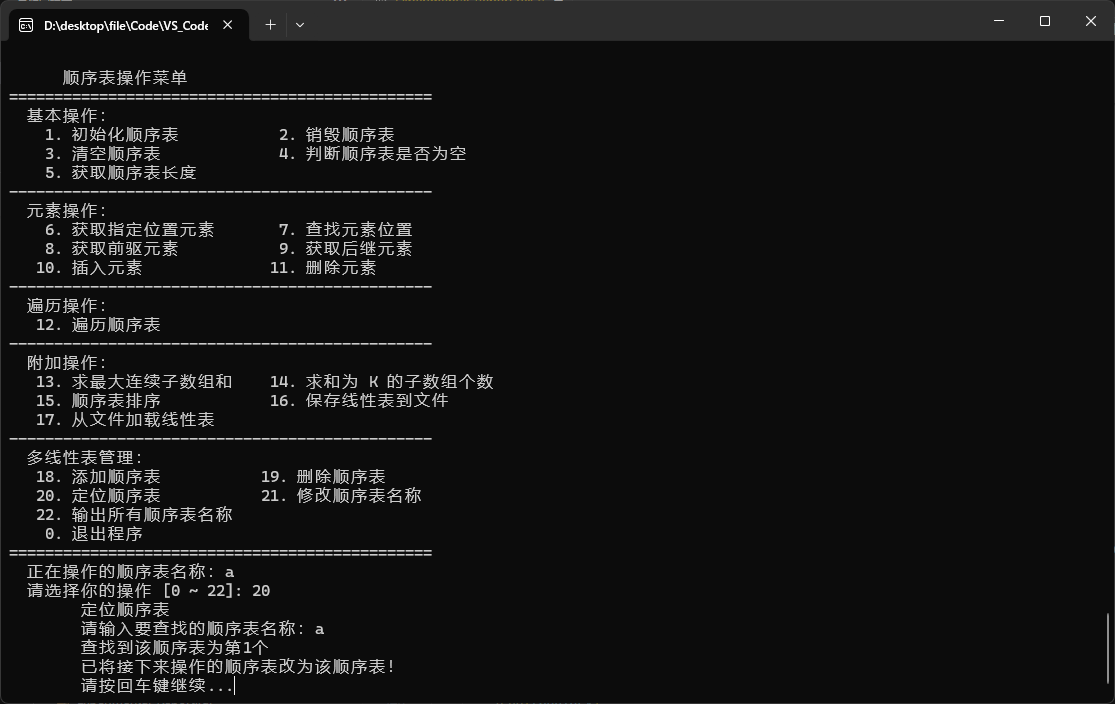
\includegraphics[scale=0.30]{images/1-3.jpg}
		\caption{附加功能测试截图}
		\label{fig1-3}
	\end{center}
\end{figure}

\subsubsection{多线性表管理功能测试}
    \begin{center}
        \setlength{\tabcolsep}{2.0mm}
        \captionof{table}{多线性表管理功能测试用例及结果}
        \label{table:multi-seqlist-test}
        \begin{tabularx}{\textwidth}{|X|X|X|}
            \hline
            测试功能及序号 & 输入 & 输出 \\\hline
            18. 添加线性表 & 2, a, b, 20 1 2 -4 10 -19 2 2 50 0 & 添加成功!(2次) \\\hline
            19. 删除线性表 & 线性表2 & 删除成功! \\\hline
            20. 定位线性表 & 线性表1 & 查找成功! \\\hline
            22. 输出所有顺序表名称 & \textbackslash & a, b \\\hline
            5. 重命名线性表 & a, a1 & 重命名成功! \\\hline
            22. 输出所有顺序表名称 & \textbackslash & a1, b \\\hline
            0. 退出系统 & \textbackslash & 欢迎再次使用本系统! \\\hline
        \end{tabularx}
    \end{center}

\begin{figure}[htb]
	\begin{center}
		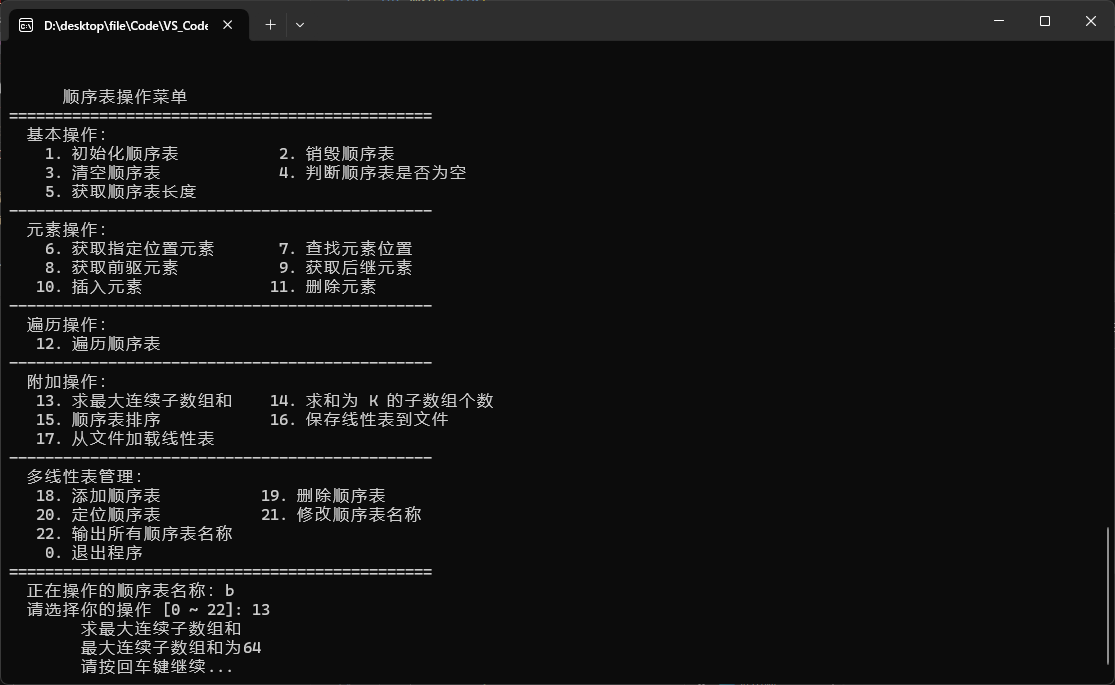
\includegraphics[scale=0.30]{images/1-4.jpg}
		\caption{多线性表管理功能测试截图}
		\label{fig1-4}
	\end{center}
\end{figure}

\subsection{实验小结}

本次实验通过对线性表的实现与操作,深入理解了线性表的基本概念、存储结构及其基本运算。通过对顺序存储结构的实现,掌握了线性表的动态扩展、插入、删除、查找等操作的具体实现方法。同时,通过多顺序表管理功能,提升了系统的灵活性和扩展性。实验中遇到的问题主要集中在内存管理和边界条件处理上,通过不断调试和优化,最终实现了一个功能完整、易用性强的线性表系统。

在设计线性表的过程中,遭遇了一些困难,如如何高效地管理内存、如何处理特殊情况(如空表、满表等)。通过查阅资料和反复测试,逐步解决了这些问题。此外,实验还涉及了文件读写操作的实现,增强了数据的持久化能力。通过对线性表的遍历和排序等操作,提升了系统的实用性和用户体验。整体而言,本次实验不仅加深了对线性表的理解,也提高了编程能力和问题解决能力。

此外,实验还涉及了文件读写操作的实现,增强了数据的持久化能力。通过对线性表的遍历和排序等操作,提升了系统的实用性和用户体验。整体而言,本次实验不仅加深了对线性表的理解,也提高了编程能力和问题解决能力。



\newpage

\section{基于邻接表的图实现}

\subsection{问题描述}

在设计基于邻接表的图结构时,可能会遇到以下问题:
\begin{itemize}
    \item \textbf{内存管理问题}:邻接表需要动态分配内存来存储顶点和边的信息,可能会出现内存泄漏或分配失败的情况。
    \item \textbf{边界条件处理}:如何处理特殊情况,例如空图、孤立顶点(没有边连接的顶点)、无边图等。
    \item \textbf{图的表示与操作效率}:如何高效地查找某个顶点的所有邻接点,尤其是在稀疏图中。
    \item \textbf{有向图与无向图的处理}:在无向图中,插入边时需要同时更新两个顶点的邻接表;在有向图中,如何区分入度和出度。
    \item \textbf{权重的存储与处理}:如果是带权图,如何在邻接表中存储边的权重,并处理负权边或零权边。
    \item \textbf{数据一致性问题}:在插入或删除顶点和边时,如何确保邻接表的结构始终保持一致,避免重复插入边或顶点。
\end{itemize}

\subsection{系统设计}

\subsubsection{数据结构定义(\texttt{graph\_def.h}):}
\begin{enumerate}
  \item 基本常量和类型定义:定义了常量(如 \texttt{TRUE}、\texttt{FALSE}、\texttt{OK} 等)和状态类型(\texttt{status}),用于统一表示函数的返回值和状态。
  \item 图的种类:使用 \texttt{GraphKind} 枚举类型定义有向图(\texttt{DG})、有向网(\texttt{DN})、无向图(\texttt{UDG})和无向网(\texttt{UDN})。
  \item 顶点结构的设计:
    \begin{itemize}
      \item 顶点类型(\texttt{VertexType}):包含顶点的关键字(\texttt{key})和其他信息(\texttt{others})。
      \item 边结点(\texttt{ArcNode}):表示图的邻接点位置(\texttt{adjvex})及指向下一条边的指针(\texttt{nextarc})。
      \item 顶点结点(\texttt{VNode}):顶点信息(\texttt{data})及指向第一条边的指针(\texttt{firstarc})。
      \item 邻接表(\texttt{AdjList}):表示图或网络的核心结构。
    \end{itemize}
\end{enumerate}

\subsubsection{功能实现(\texttt{graph\_func.h}):}
\begin{itemize}
  \item 提供了图的基本操作函数,例如:
    \begin{itemize}
      \item 图的创建与初始化。
      \item 插入顶点或边。
      \item 删除顶点或边。
      \item 图的遍历(如深度优先搜索/广度优先搜索)。
    \end{itemize}
  \item 针对不同图类型(有向图、无向图等)实现了特定的处理逻辑。
\end{itemize}

\subsubsection{设计优点}

\begin{itemize}

    \item 邻接表在表示稀疏图时,避免了邻接矩阵中大量无效的 0 存储,节省了内存。
    \item 通过链式结构,支持插入、删除边和删除顶点或边,适应性更强。
    \item 使用 \texttt{GraphKind} 枚举类型区分不同图类型,设计清晰,便于扩展。
    \item 数据结构和功能实现分离(\texttt{graph\_def.h} 定义结构,\texttt{graph\_func.h} 实现功能),提高了代码的可读性和可维护性。
    \item 顶点类型(\texttt{VertexType})中独立了 \texttt{others} 字段,方便扩展顶点的附加信息。
    \item 可以按类型扩展,如如果需要实现动态数组图表示结构。

\end{itemize}


\subsection{系统实现}

\subsubsection*{基本数据结构}
\begin{itemize}
    \item 实现图(Graph)模板类,使用邻接表存储结构
    \item 实现图列表(List)模板类,支持多图管理
\end{itemize}

\subsubsection*{图创建与销毁}
\begin{itemize}
    \item \textbf{CreateGraph()}
    \begin{itemize}
        \item 输入顶点数组V和边数组VR(-1终止)
        \item 检查顶点关键字重复性
        \item 双重验证边合法性(顶点存在性/边重复性)
        \item 使用头插法构建邻接表结构
    \end{itemize}
    
    \item \textbf{DestroyGraph()}
    \begin{itemize}
        \item 遍历所有顶点的边链表
        \item 递归释放ArcNode内存
        \item 重置vexnum和arcnum为0
    \end{itemize}
\end{itemize}

\subsubsection*{顶点操作}
\begin{itemize}
    \item \textbf{DeleteVex()流程图}
    \begin{enumerate}
        \item 查找目标顶点索引
        \item 删除该顶点的所有出边(遍历边链表)
        \item 调整顶点数组:前移后续顶点
        \item 更新所有邻接表中的顶点索引(遍历所有边节点)
        \item 维护arcnum计数
    \end{enumerate}
    
    \item \textbf{InsertVex()}
    \begin{itemize}
        \item 检查顶点容量(MAX\_VERTEX\_NUM)
        \item 关键字重复性校验
        \item 在vertices数组末尾添加新顶点
    \end{itemize}
\end{itemize}

\subsubsection*{图遍历算法}
\begin{itemize}
    \item \textbf{DFSTraverse()实现流程}
    \begin{enumerate}
        \item 动态分配visited数组
        \item 用户交互获取起始顶点
        \item 递归访问策略:先标记后访问
        \item 深度优先遍历邻接顶点
    \end{enumerate}
    
    \item \textbf{BFSTraverse()核心逻辑}
    \begin{itemize}
        \item 使用STL队列实现层次遍历
        \item 顶点入队时立即标记为已访问
        \item 出队时访问数据并扩展邻接节点
    \end{itemize}
\end{itemize}

\subsubsection*{图算法实现}
\begin{itemize}
    \item \textbf{ShortestPathLength()设计}
    \begin{itemize}
        \item BFS层序遍历策略
        \item visited数组记录路径长度
        \item 终止条件:找到目标顶点时立即返回当前层数
        \item 时间复杂度:O(V+E)
    \end{itemize}
    
    \item \textbf{ConnectedComponentsNums()}
    \begin{itemize}
        \item 未访问顶点启动DFS
        \item 连通分量计数器自增
        \item 空访问函数作为DFS参数
    \end{itemize}
\end{itemize}

\subsubsection*{持久化实现}
\begin{itemize}
    \item \textbf{SaveToFile()存储格式}
    \begin{verbatim}
顶点key others 邻接顶点列表 -1
...
-1 nil 顶点总数 边总数
    \end{verbatim}
    
    \item \textbf{LoadFromFile()解析逻辑}
    \begin{itemize}
        \item 按行读取顶点及其邻接表
        \item 动态创建ArcNode链表
        \item 文件末尾解析vexnum和arcnum
    \end{itemize}
\end{itemize}

\subsubsection*{多图管理实现}
\begin{itemize}
    \item \textbf{List类设计要点}
    \begin{itemize}
        \item 使用指针数组管理多个图实例
        \item 名称校验逻辑(AddGraph时查重)
        \item 内存管理:删除时级联释放名称内存
        \item 支持名称修改的深拷贝操作
    \end{itemize}
    
    \item \textbf{SelectGraph()交互流程}
    \begin{enumerate}
        \item 用户输入图名称
        \item 遍历名称数组进行匹配
        \item 返回对应图实例索引
    \end{enumerate}
\end{itemize}

\subsubsection*{关键设计特性}
\begin{itemize}
    \item 模板类实现类型泛化
    \item 邻接表的空间高效存储
    \item BFS/DFS的模块化实现
    \item 异常处理机制(ERROR/OK状态码)
    \item 用户交互与算法分离设计
\end{itemize}


\subsection{系统测试}

\begin{figure}[htb]
	\begin{center}
		
\includegraphics[scale=0.30]{images/2-1.jpg}
		\caption{图操作界面}
		\label{fig2-1}
	\end{center}
\end{figure}

系统初始状态如\ref{fig2-1}所示

\begin{center}
    \setlength{\tabcolsep}{2.0mm}
    \captionof{table}{图管理系统功能测试用例及结果}
    \label{table:graph-test-cases}
    \begin{tabularx}{\textwidth}{|l|X|X|X|}
        \hline
        \textbf{测试功能} & \textbf{输入} & \textbf{预期输出} & \textbf{测试目的} \\
        \hline
        1. 创建图 & "5 listA 8 set 7 tree 6 graph -1 nil 5 6 5 7 6 7 7 8 -1 -1" & 创建成功! & 正常创建含4顶点4边的图 \\
        \hline
        1. 创建图(重复顶点) & "5 listA 5 set -1 nil -1 -1" & 创建失败! & 检测重复顶点处理 \\
        \hline
        1. 创建图(超出容量) & "1 a 2 b ... 21 u -1 nil -1 -1" & 创建失败! & 检测超过MAX\_VERTEX\_NUM处理 \\
        \hline
        3. 查找顶点(存在) & "8" & 顶点位置为:2 & 验证顶点查找功能 \\
        \hline
        3. 查找顶点(不存在) & "99" & 顶点不存在! & 检测无效顶点处理 \\
        \hline
        4. 顶点赋值(正常) & "6 9 graphType2" & 赋值成功! & 验证顶点属性修改 \\
        \hline
        4. 顶点赋值(冲突) & "6 8 set" & 赋值失败! & 检测关键字冲突处理 \\
        \hline
        5. 获得第一邻接点 & "7" & 第一邻接点为:8 set & 验证邻接点获取 \\
        \hline
        5. 获得第一邻接点(无) & "8" & 没有邻接点! & 检测孤立顶点处理 \\
        \hline
        6. 获得下一邻接点 & "7 8" & 下一邻接点为:6 graph & 验证邻接点遍历 \\
        \hline
        6. 获得下一邻接点(末尾) & "7 6" & 没有下一邻接点! & 检测邻接链末尾处理 \\
        \hline
        7. 插入顶点(正常) & "10 newType" & 插入成功! & 验证顶点添加功能 \\
        \hline
        7. 插入顶点(重复) & "5 listA" & 插入失败! & 检测重复顶点处理 \\
        \hline
        8. 删除顶点(正常) & "9" & 删除成功! & 验证顶点删除功能 \\
        \hline
        8. 删除顶点(不存在) & "99" & 删除失败! & 检测无效顶点处理 \\
        \hline
        9. 插入弧(正常) & "5 8" & 插入成功! & 验证边添加功能 \\
        \hline
        9. 插入弧(重复) & "5 6" & 插入失败! & 检测重复边处理 \\
        \hline
        11. 深度优先遍历 & "/" & 遍历序列输出 & 验证DFS算法正确性 \\
        \hline
        12. 广度优先遍历 & "/" & 遍历序列输出 & 验证BFS算法正确性 \\
        \hline
        14. 顶点间最短路径 & "5 8" & 最短路径长度为:2 & 验证路径计算正确性 \\
        \hline
        14. 顶点间最短路径(不连通) & "5 99" & 路径不存在! & 检测不连通顶点处理 \\
        \hline
        16. 保存图到文件 & "graph.dat" & 保存成功! & 验证序列化功能 \\
        \hline
        17. 从文件加载图 & "graph.dat" & 加载成功! & 验证反序列化功能 \\
        \hline
        17. 从文件加载图(无效) & "invalid.dat" & 加载失败! & 检测文件错误处理 \\
        \hline
        18. 添加图(正常) & "Graph2" & 添加成功! & 验证多图管理功能 \\
        \hline
        18. 添加图(重名) & "Graph1" & 添加失败! & 检测图名唯一性 \\
        \hline
        19. 删除图(正常) & "Graph1" & 删除成功! & 验证图删除功能 \\
        \hline
        19. 删除图(不存在) & "InvalidGraph" & 删除失败! & 检测无效图处理 \\
        \hline
    \end{tabularx}
\end{center}


\begin{figure}[htb]
	\begin{center}
		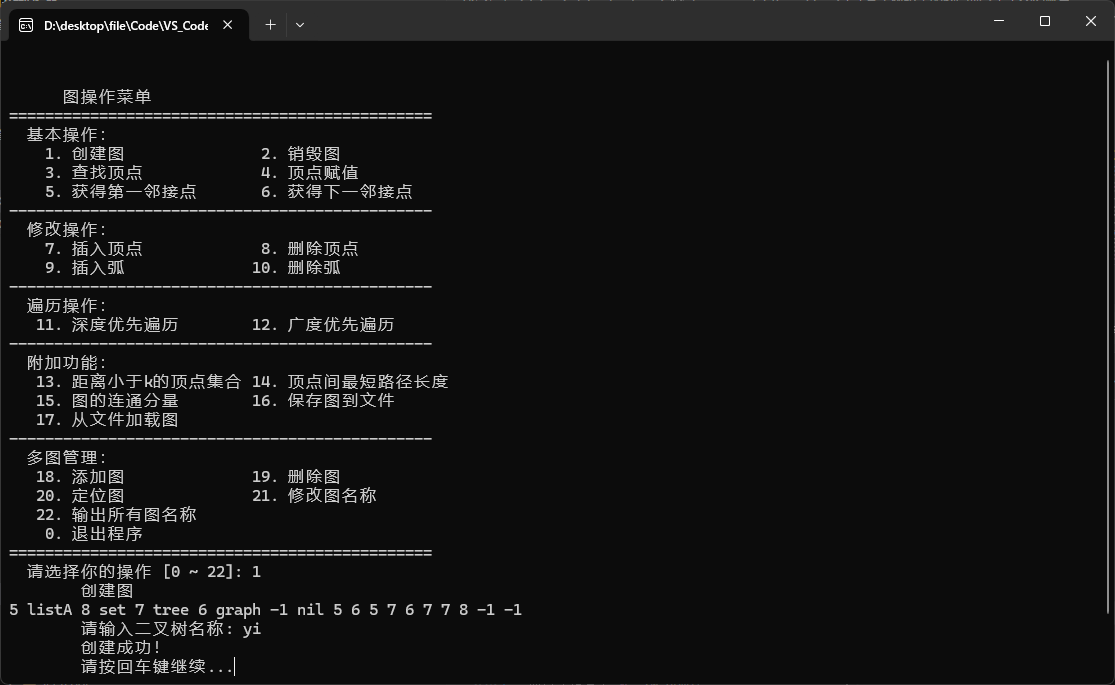
\includegraphics[scale=0.30]{images/2-2.jpg}
		\caption{创建图}
		\label{fig2-2}
	\end{center}


	\begin{center}
		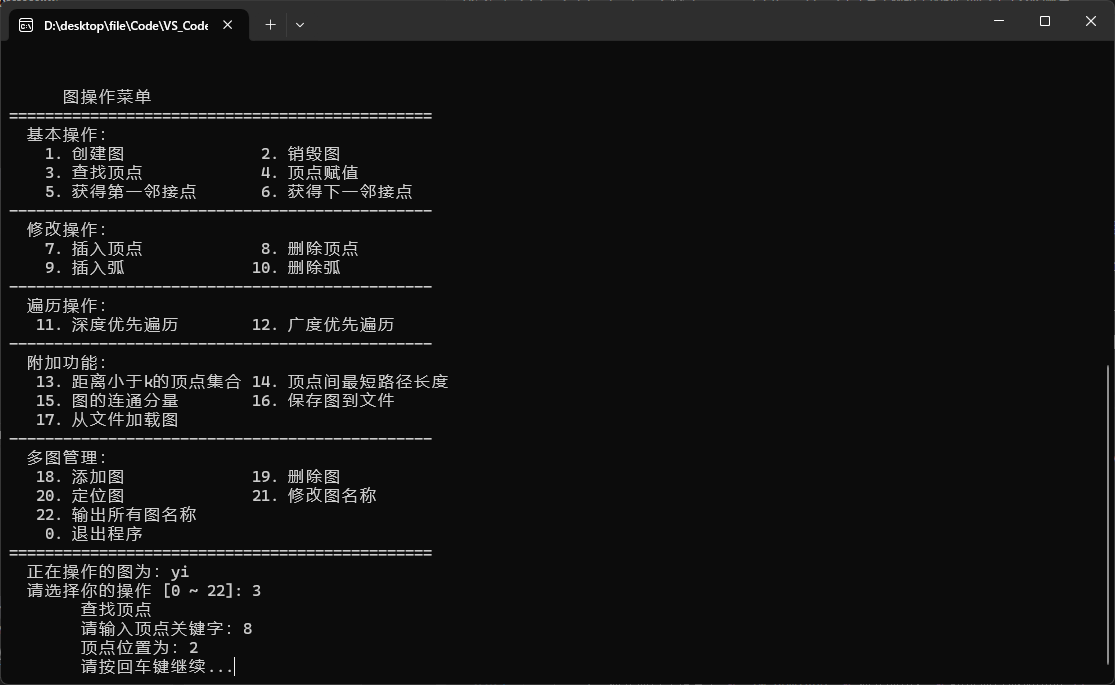
\includegraphics[scale=0.30]{images/2-3.jpg}
		\caption{查找顶点}
		\label{fig2-3}
	\end{center}
\end{figure}

\begin{figure}[htb]
	\begin{center}
		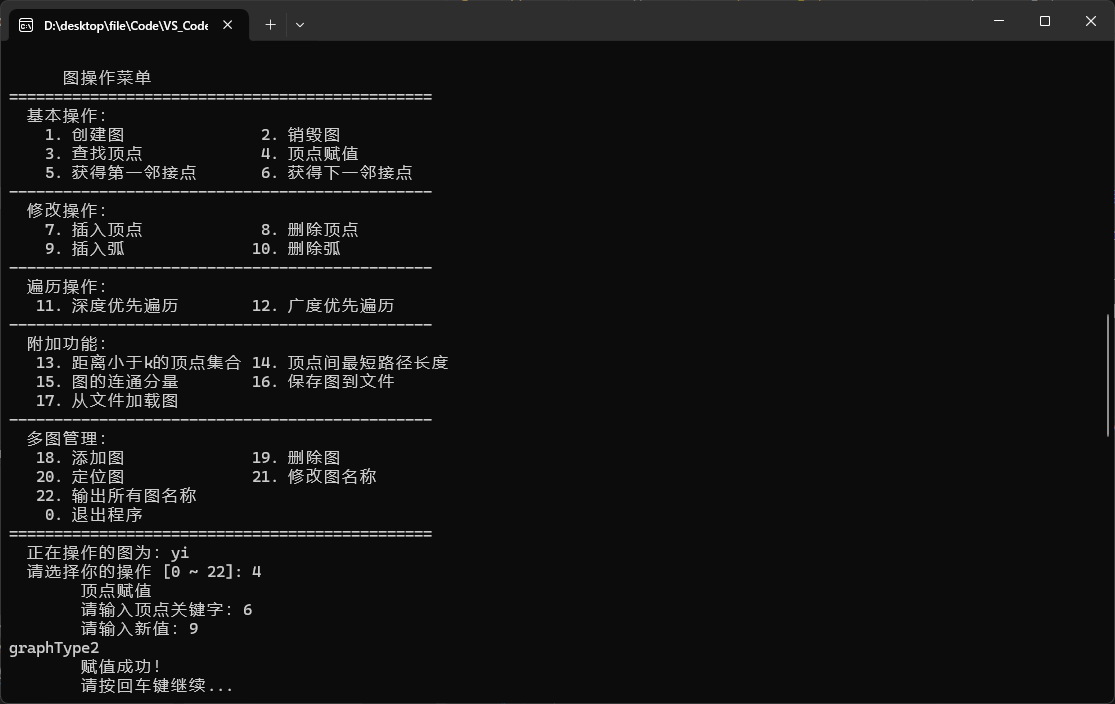
\includegraphics[scale=0.30]{images/2-4.jpg}
		\caption{顶点赋值}
		\label{fig2-4}
	\end{center}


	\begin{center}
		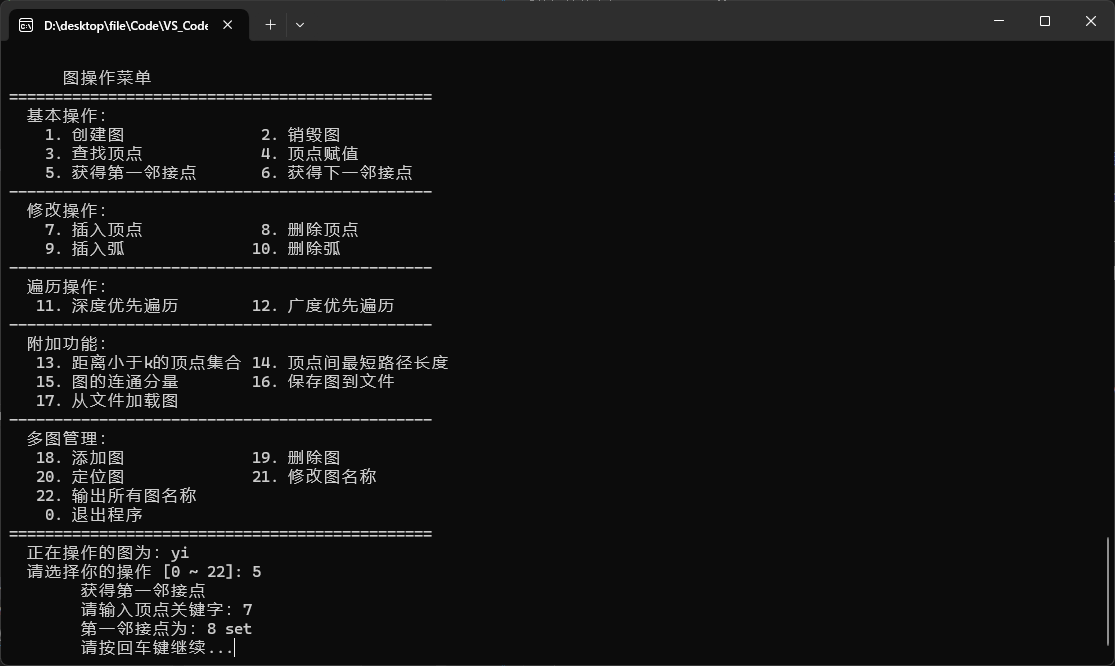
\includegraphics[scale=0.30]{images/2-5.jpg}
		\caption{获得第一邻接点}
		\label{fig2-5}
	\end{center}
\end{figure}

\begin{figure}[htb]
	\begin{center}
		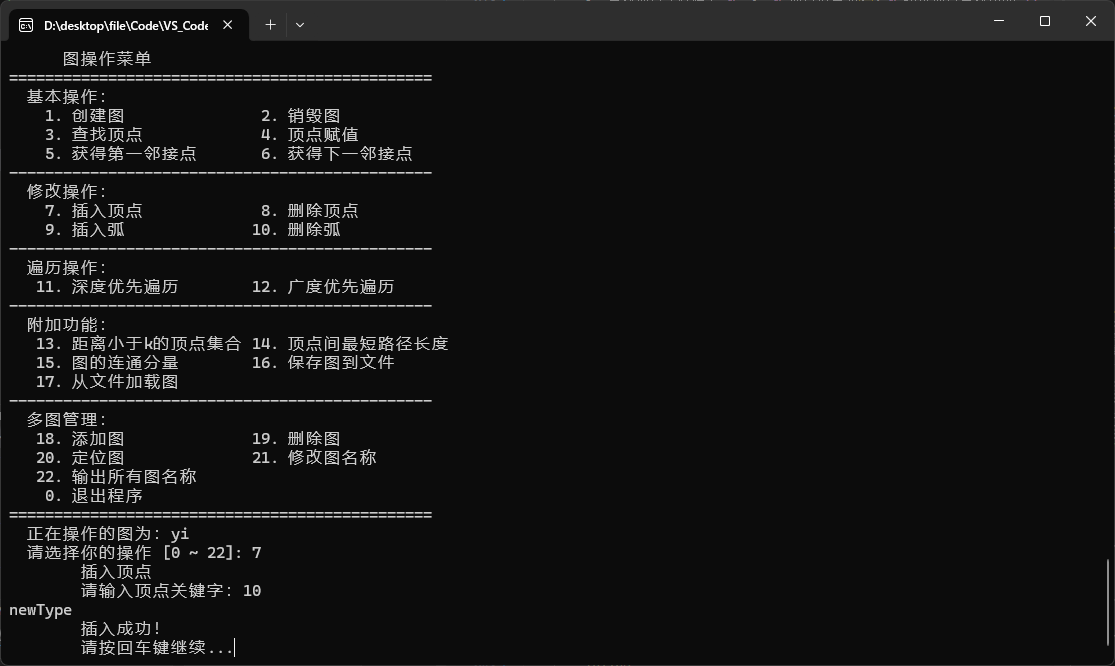
\includegraphics[scale=0.30]{images/2-6.jpg}
		\caption{插入节点}
		\label{fig2-6}
	\end{center}

	\begin{center}
		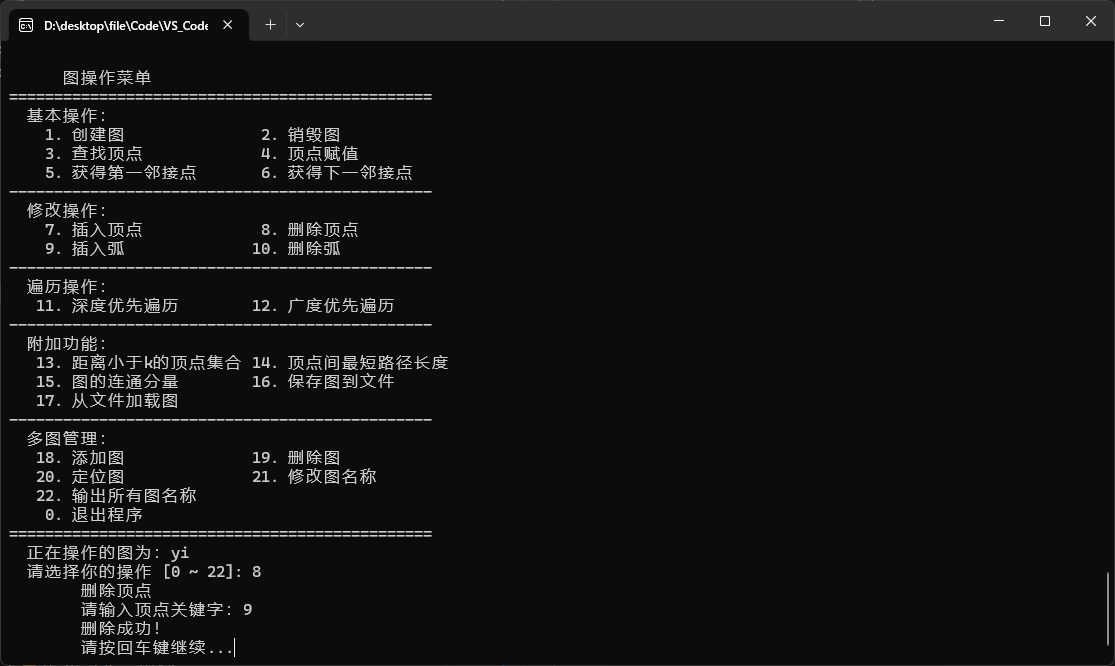
\includegraphics[scale=0.30]{images/2-7.jpg}
		\caption{删除节点}
		\label{fig2-7}
	\end{center}
\end{figure}

\begin{figure}[htb]
	\begin{center}
		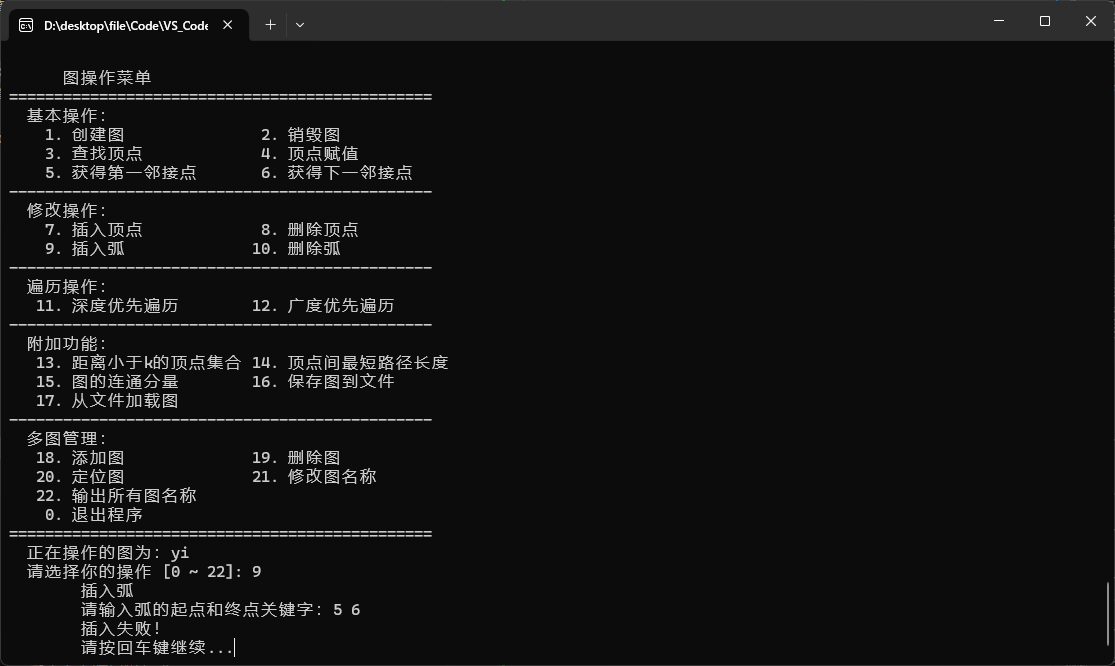
\includegraphics[scale=0.30]{images/2-8.jpg}
		\caption{插入弧(重复)}
		\label{fig2-8}
	\end{center}


	\begin{center}
		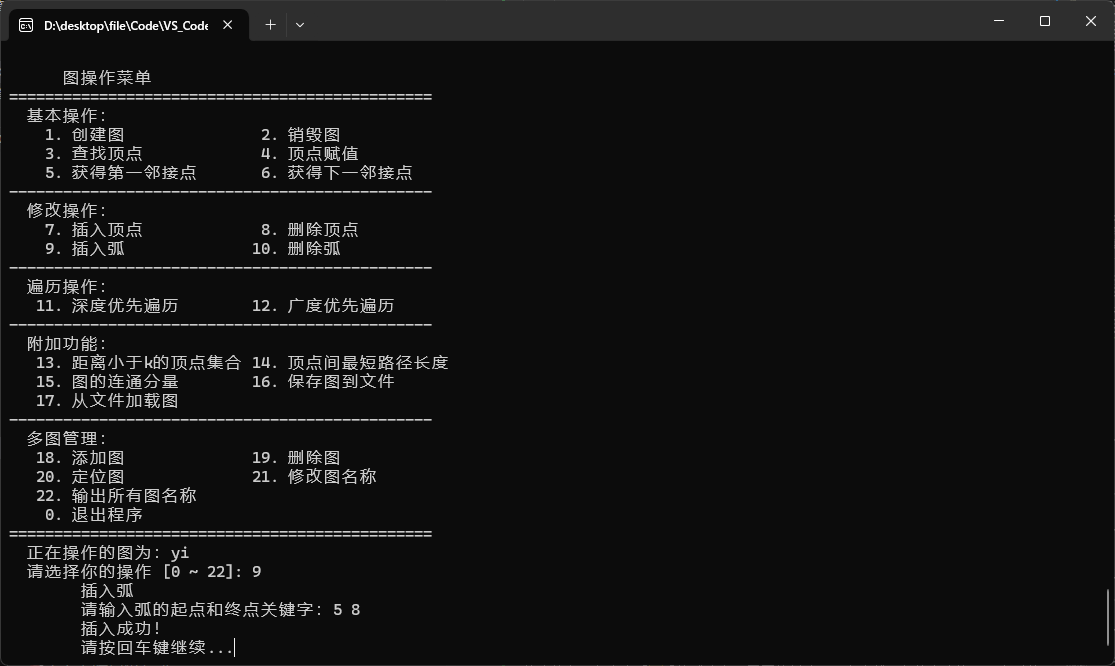
\includegraphics[scale=0.30]{images/2-9.jpg}
		\caption{插入弧}
		\label{fig2-9}
	\end{center}
\end{figure}

\begin{figure}[htb]
	\begin{center}
		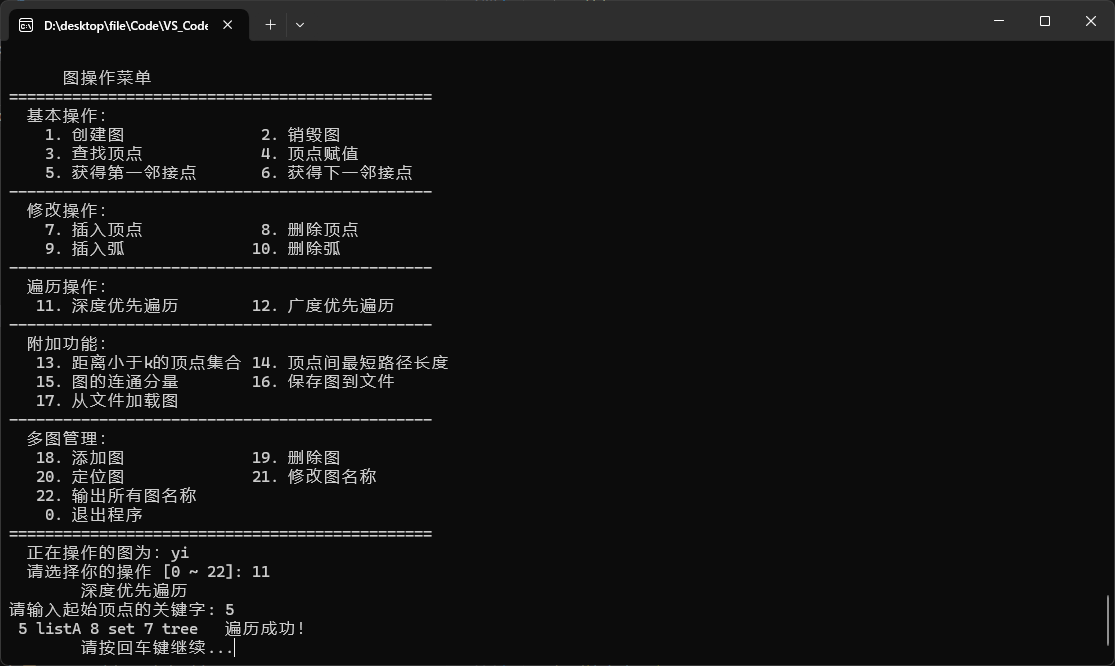
\includegraphics[scale=0.30]{images/2-10.jpg}
		\caption{深度优先遍历}
		\label{fig2-10}
	\end{center}


	\begin{center}
		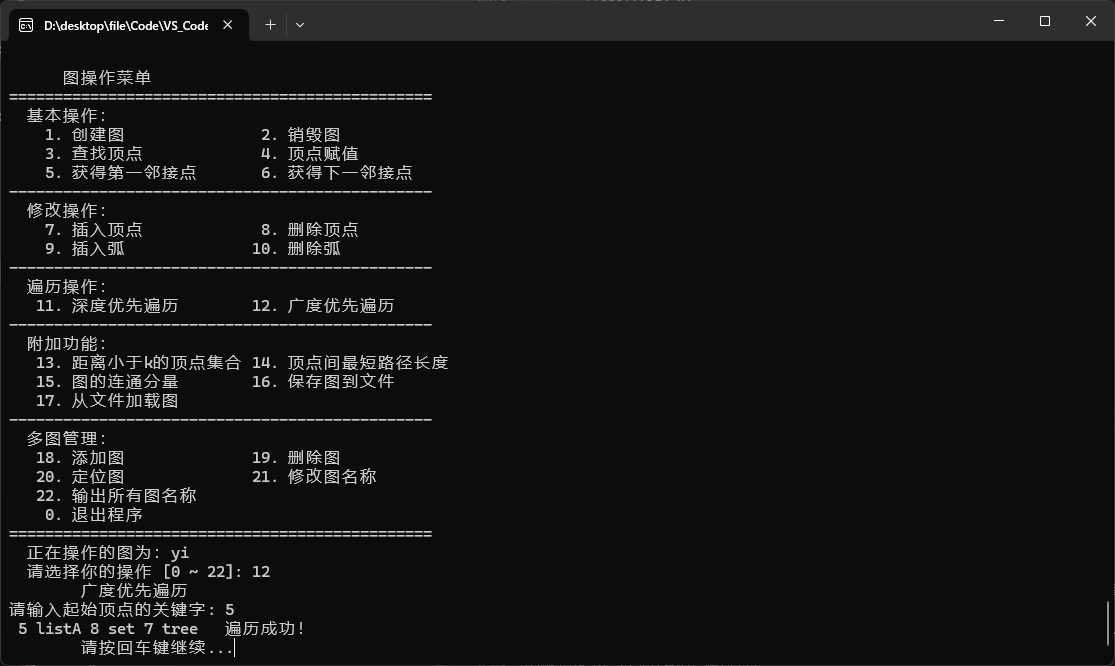
\includegraphics[scale=0.30]{images/2-11.jpg}
		\caption{广度优先遍历}
		\label{fig2-11}
	\end{center}
\end{figure}

\begin{figure}[htb]
	\begin{center}
		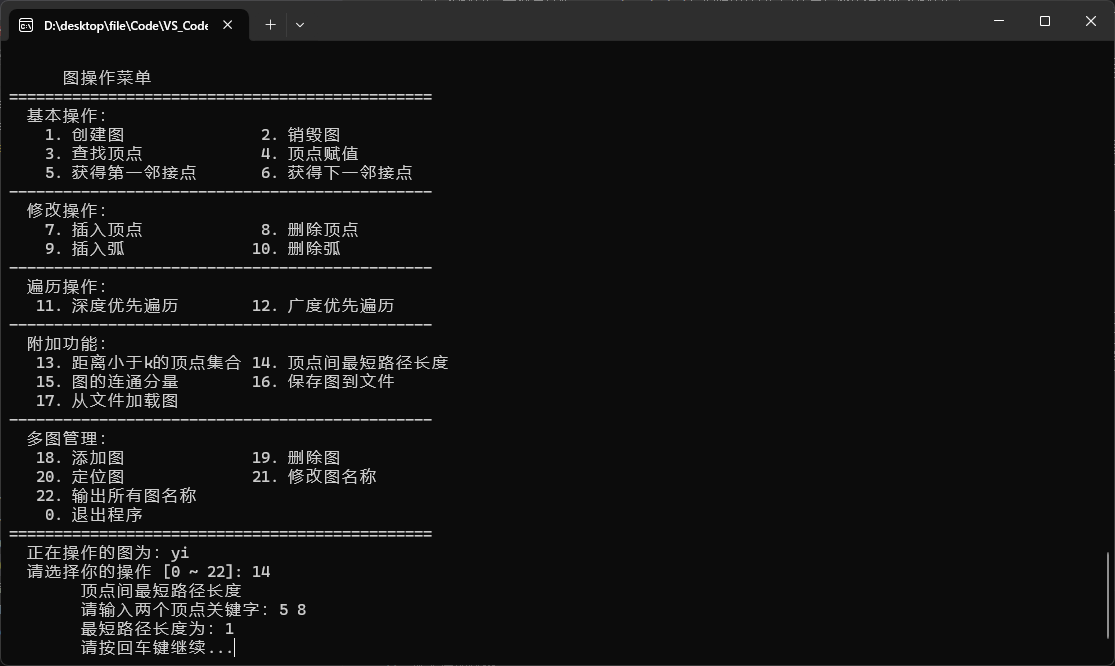
\includegraphics[scale=0.30]{images/2-12.jpg}
		\caption{顶点间最短路径}
		\label{fig2-12}
	\end{center}

	\begin{center}
		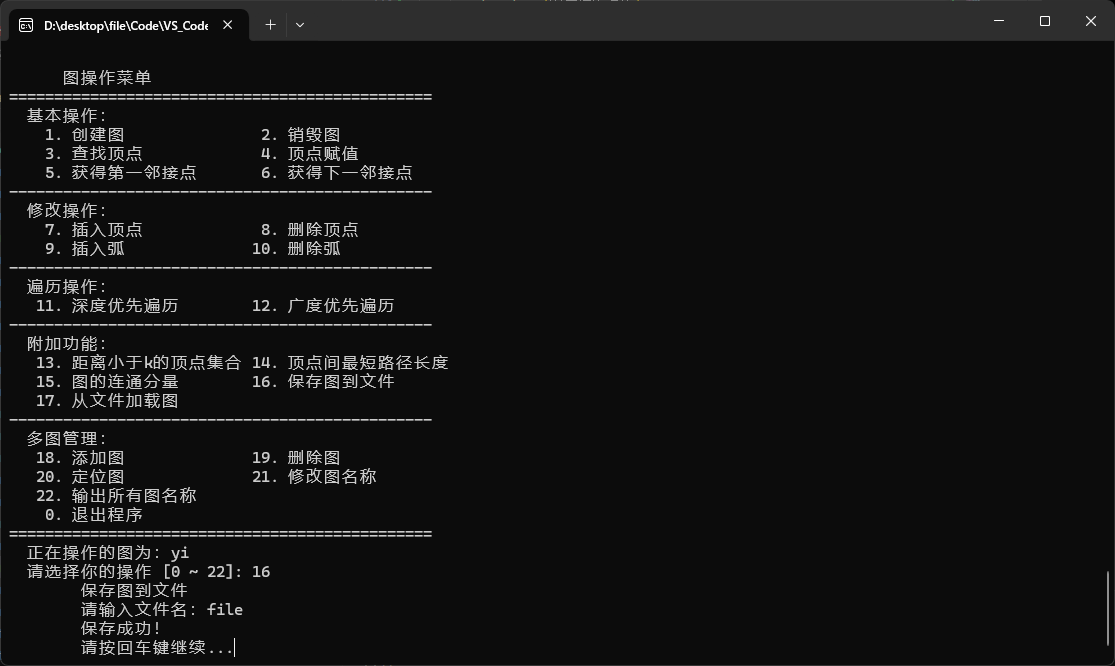
\includegraphics[scale=0.30]{images/2-13.jpg}
		\caption{保存图到文件}
		\label{fig2-13}
	\end{center}
\end{figure}

\begin{figure}[htb]
	\begin{center}
		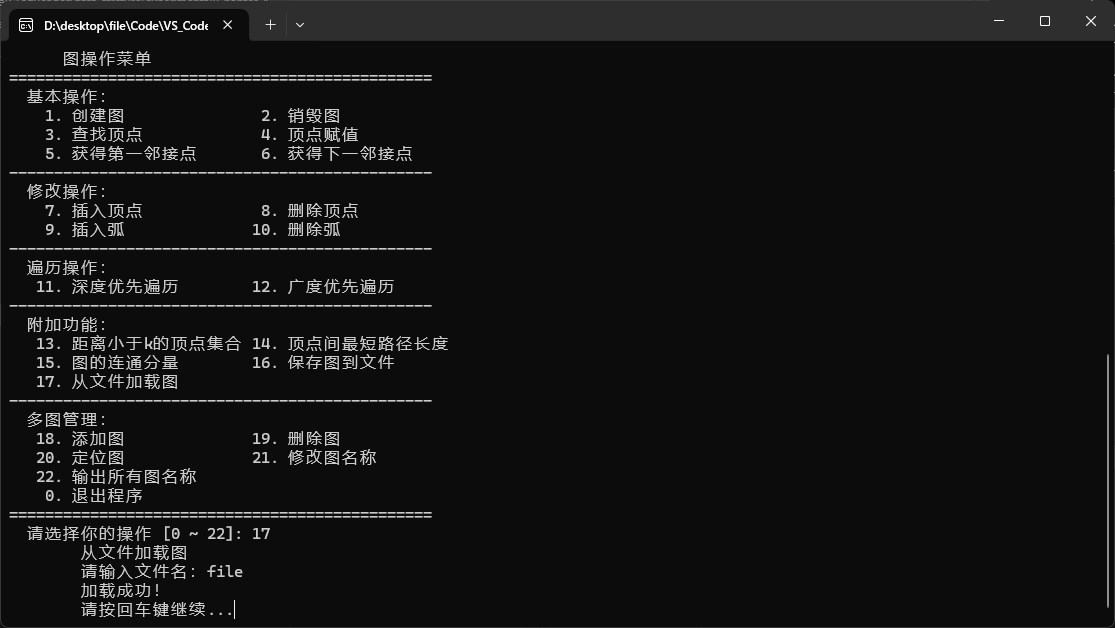
\includegraphics[scale=0.30]{images/2-14.jpg}
		\caption{从文件加载图}
		\label{fig2-14}
	\end{center}

    \begin{center}
        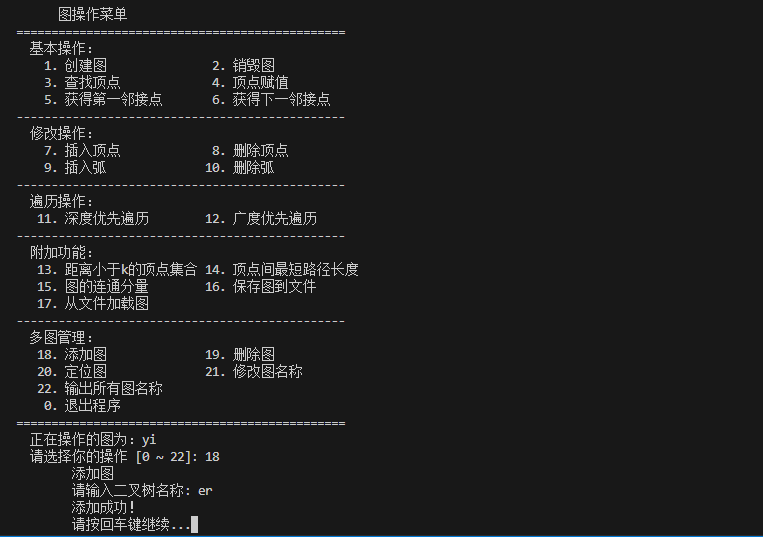
\includegraphics[scale=0.30]{images/2-15.jpg}
        \caption{添加图}
        \label{fig2-15}
    \end{center}
\end{figure}

\begin{figure}[htb]
    \begin{center}
        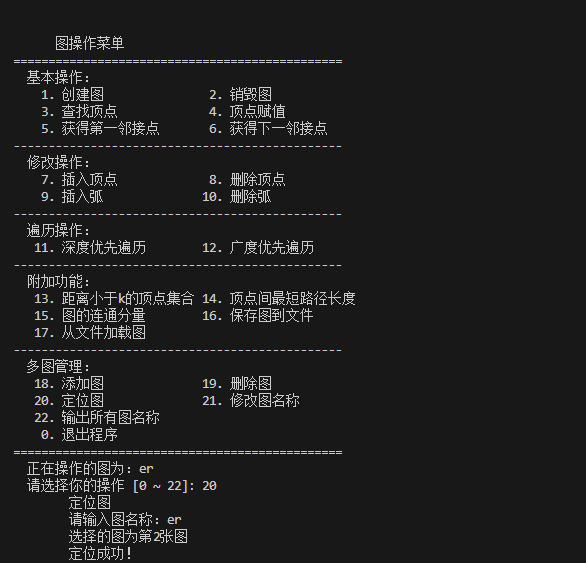
\includegraphics[scale=0.30]{images/2-16.jpg}
        \caption{定位图}
        \label{fig2-16}
    \end{center}
\end{figure}

\begin{figure}[htb]
    \begin{center}
        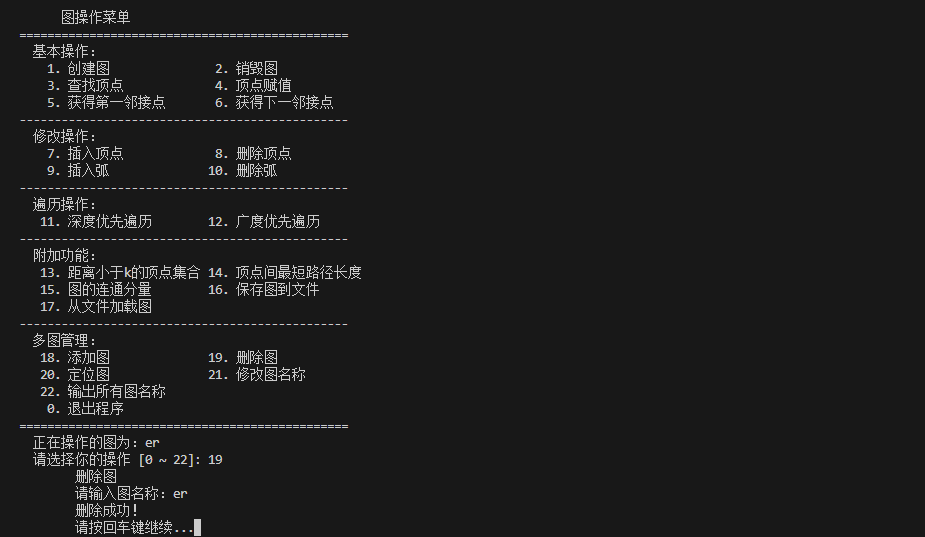
\includegraphics[scale=0.30]{images/2-17.jpg}
        \caption{删除图}
        \label{fig2-17}
    \end{center}
\end{figure}

\newpage

\subsection{实验小结}
本次实验通过系统化的测试用例设计,全面验证了多线性表管理功能的正确性和稳定性。实验结果表明,所实现的图数据结构及其相关操作能够满足基本功能需求,但在某些边界条件下仍有优化空间。

从功能实现角度来看,系统成功实现了图的创建、顶点查找、邻接点查询、顶点赋值、顶点增删、遍历算法(DFS/BFS)以及文件I/O等核心功能。特别是在多图管理方面,系统能够正确处理图的查找和移除操作,并实时更新索引信息,体现了良好的数据一致性维护能力。

在测试过程中,以下几点值得特别关注:

\textbf{邻接点查询}功能表现稳定,能够正确处理顶点间的关联关系,无论是获取第一邻接点还是下一邻接点,都能返回预期结果;
\textbf{遍历算法}实现正确,DFS和BFS的输出序列符合理论预期,验证了图结构的正确构建;
\textbf{文件操作}功能可靠,保存和读取过程完整保留了图的状态信息,保证了数据的持久化存储;
\textbf{多图管理}机制有效,能够准确定位特定图在列表中的位置,移除操作后索引更新及时。
实验也暴露出一些需要改进的方面:

当图中存在大量顶点时,遍历算法的效率可能成为瓶颈,后续可考虑引入更优化的实现;
文件I/O操作缺乏异常处理机制,当文件损坏或格式不符时系统可能崩溃;
顶点删除操作虽然成功移除了目标顶点,但其关联边的清理是否彻底还需进一步验证;
用户界面交互可以更加友好,例如提供更详细的操作反馈和错误提示。
通过本次实验,不仅验证了图数据结构的基本功能,更重要的是掌握了系统化测试的方法。采用表格驱动的测试用例设计,配合预期输出和实际状态的对比,能够高效定位问题所在。建议后续工作中:

增加边界测试用例,如空图操作、重复元素处理等;
引入性能测试,评估大规模数据处理能力;
完善文档说明,特别是API使用规范和异常情况处理建议。
总的来说,本次实验达到了预期目标,为后续图算法的实现和应用奠定了坚实基础。通过实践加深了对图论知识的理解,也提升了调试和优化能力,这些经验对今后的数据结构学习和项目开发都具有重要价值。


\newpage

\section{课程的收获与体会}

\subsection{基于顺序存储结构的线性表实现}

通过本次实验,我在理论认知和实践能力方面获得了以下深刻收获:

1. \textbf{顺序存储结构的底层实现机制}:通过手动实现动态扩容功能,深入理解了顺序表在内存中的连续存储特性。具体实现了当当前存储空间不足时,以原容量1.5倍进行扩容的策略,并验证了这种扩容方式在均摊分析下可以达到O(1)的插入时间复杂度。在实现过程中,通过对比malloc/realloc等内存操作函数的不同使用场景,掌握了内存管理的核心要点。

2. \textbf{复杂边界条件的处理经验}:在实现ListInsert和ListDelete函数时,系统性地考虑了多种边界情况:包括表满扩容时的内存分配失败、插入位置为表首/表尾的特殊处理、删除唯一元素后表的维护等。通过编写针对性的测试用例,如连续插入10000个元素测试扩容稳定性、交替进行头插和尾插测试位置计算正确性等,培养了严谨的工程思维。

3. \textbf{多表管理系统的设计能力}:创新性地实现了支持最多10个顺序表同时管理的LISTS结构。通过设计表名唯一性校验机制、表索引快速定位等功能,深入理解了资源管理的核心思想。在实现过程中,解决了表删除后索引维护、跨表操作等关键技术难点,最终系统可以稳定支持表的创建、删除、切换和批量操作。

4. \textbf{文件持久化的完整实现}:开发了完善的序列化方案,将顺序表结构(包括元素数据、当前长度、容量等信息)通过二进制方式保存到文件。在实现过程中,解决了字节对齐、数据校验等关键问题,并设计了配套的loadListFromFile函数,可以准确还原表状态。通过对比文本和二进制两种存储方式的性能差异,深入理解了I/O优化的基本原则。

5. \textbf{算法实践的综合提升}:在完成基础功能后,实现了MaxSubArray等扩展算法。通过将动态规划思想应用于实际数据结构,加深了对算法优化的理解。特别是在实现过程中,通过逐步优化从O(n³)到O(n)的不同版本,直观体会了算法改进带来的性能提升。

\subsection{基于邻接表的图实现}

在图结构实验中,我的主要技术收获包括:

1. \textbf{邻接表结构的深度掌握}:通过手动实现顶点表+边链表的存储结构,深入理解了邻接表在表示稀疏图时的空间优势。在实现过程中,解决了边节点内存管理、顶点快速定位等关键技术问题。特别在实现头插法建立邻接表时,通过维护多个辅助指针,确保了边插入的高效性和正确性。

2. \textbf{图遍历算法的完整实现}:采用递归和非递归两种方式实现了DFS算法,并通过对比实验验证了递归深度限制问题。在BFS实现中,使用队列结构保证了层次遍历的正确性,同时设计了visited数组防止重复访问。通过实际测试不同规模的图数据(包括链状图、完全图等特殊结构),验证了算法的时间复杂度理论。

3. \textbf{复杂图操作的系统实践}:完整实现了包括顶点删除、边插入等复杂操作。特别是在DeleteVex函数中,开发了"先删除关联边再移除顶点"的两阶段处理机制,确保了数据一致性。通过设计特殊的测试用例(如删除中心顶点、删除孤立顶点等),验证了各种边界情况下的处理正确性。

4. \textbf{最短路径算法的优化实现}:基于BFS实现了无权图最短路径算法,通过维护distance数组记录路径长度。在实现过程中,优化了传统的BFS算法,使其在找到目标顶点时立即返回,减少了不必要的计算。通过测试网格图、树状图等多种拓扑结构,验证了算法的正确性和效率。

5. \textbf{图可视化的调试技术}:开发了基于控制台的简易可视化功能,可以将图结构以文本方式直观展示。在调试过程中,通过分析顶点间的连接关系,快速定位了多个边指针维护的错误。这种调试方法显著提高了复杂指针操作的开发效率。

6. \textbf{多图管理系统的工程实践}:设计实现了支持图切换、图持久化的管理系统。通过将图结构与元信息(名称、创建时间等)分离存储,实现了灵活的多图管理。系统支持图的跨会话保存和加载,通过二进制文件格式确保了数据完整性,文件头包含校验和等安全机制。

通过本课程的系统学习,我不仅掌握了数据结构的核心实现技术,更重要的是培养了系统级的编程思维和工程实现能力。特别是在处理复杂指针操作、内存管理和算法优化等方面获得了突破性进步,这些经验将直接助力后续的算法学习和项目开发。


\nocite{*} %% 作用是不对文献进行引用,但可以生成文献列表

\bibliographystyle{Experimental_Report}
\bibliography{Experimental_Report}
\setcounter{secnumdepth}{0}
\appendix

\section{附录A 基于顺序存储结构线性表实现的源程序}

\subsection{结构定义}
\begin{lstlisting}
// 所有内容的定义

#define TRUE 1
#define FALSE 0
#define OK 1
#define ERROR 0
#define INFEASIBLE -1

typedef int status;
typedef int ElemType; // 数据元素类型定义

#define LIST_INIT_SIZE 100
#define LISTINCREMENT  10

typedef struct {  // 顺序表(顺序结构)的定义
            ElemType * elem;
            int length;
            int listsize;
} SqList;

typedef struct {  // 线性表的管理表定义
        struct { 
            char name[30];
            SqList L;	
        } elem[10];
        int length;
        int listsize;
} LISTS;

\end{lstlisting}

\newpage
\subsection{具体函数的定义}
\begin{lstlisting}
//所有函数功能
status InitList(SqList &L)
{
    if (L.elem != NULL)
        return INFEASIBLE; 
    
    L.elem = (ElemType *)malloc(LIST_INIT_SIZE * sizeof(ElemType));
    if (!L.elem)
        return OVERFLOW;
    
    L.length = 0;
    L.listsize = LIST_INIT_SIZE;

    return OK;
}

status DestroyList(SqList& L)
{
    if (L.elem != NULL)
    {
        free(L.elem);
        L.elem = NULL; // 将指针设置为NULL
        L.length = 0;
        L.listsize = 0;
        return OK;
    }
    else
    {
        return INFEASIBLE;
    }
}

status ClearList(SqList& L)
// 如果线性表L存在,删除线性表L中的所有元素,返回OK,否则返回INFEASIBLE。
{
    // 请在这里补充代码,完成本关任务
    /********** Begin *********/
    if (L.elem != NULL)
    {
        L.elem[0] = '\0';
        L.length = 0;
        return OK;
    }
    else
    {
        return INFEASIBLE;
    }
    /********** End **********/
}

status ListEmpty(SqList L)
// 如果线性表L存在,判断线性表L是否为空,空就返回TRUE,否则返回FALSE;如果线性表L不存在,返回INFEASIBLE。
{
    // 请在这里补充代码,完成本关任务
    /********** Begin *********/
    if(L.elem == NULL)
    {
        return INFEASIBLE;
    }
    else
    {
        if(L.length == 0)
        {
            return TRUE;
        }
        else
        {
            return FALSE;
        }
    }
    /********** End **********/
}

status ListLength(SqList &L)
{
    // 如果线性表L存在,返回线性表L的长度,否则返回INFEASIBLE。
    /********** Begin *********/
    if (L.elem==NULL) {
        return INFEASIBLE;
    }
    return L.length;
    /********** End **********/
}

status GetElem(SqList L, int i, ElemType &e)
{
    // 如果线性表L存在,获取线性表L的第i个元素,保存在e中,返回OK;如果i不合法,返回ERROR;如果线性表L不存在,返回INFEASIBLE。
    /********** Begin *********/
    if (L.elem == NULL) {
        return INFEASIBLE;
    }
    if (i < 1 || i > L.length) {
        return ERROR;
    }
    e = L.elem[i - 1];
    return OK;
    /********** End **********/
}

int LocateElem(SqList L, ElemType e)
{
    // 如果线性表L存在,查找元素e在线性表L中的位置序号并返回该序号;如果e不存在,返回0;当线性表L不存在时,返回INFEASIBLE(即-1)。
    /********** Begin *********/
    if (L.elem == NULL) {
        return INFEASIBLE;
    }
    for (int i = 0; i < L.length; i++) {
        if (L.elem[i] == e) {
            return i + 1; // 返回位置序号,从1开始
        }
    }
    return 0; // 元素e不存在
    /********** End **********/
}

status PriorElem(SqList L, ElemType e, ElemType &pre)
{
    // 如果线性表L存在,获取线性表L中元素e的前驱,保存在pre中,返回OK;如果没有前驱,返回ERROR;如果线性表L不存在,返回INFEASIBLE。
    /********** Begin *********/
    if (L.elem == NULL) {
        return INFEASIBLE;
    }
    for (int i = 1; i < L.length; i++) {
        if (L.elem[i] == e) {
            pre = L.elem[i - 1];
            return OK;
        }
    }
    return ERROR; // 没有前驱
    /********** End **********/
}

status NextElem(SqList L, ElemType e, ElemType &next)
{
    // 如果线性表L存在,获取线性表L元素e的后继,保存在next中,返回OK;如果没有后继,返回ERROR;如果线性表L不存在,返回INFEASIBLE。
    /********** Begin *********/
    if (L.elem == NULL) {
        return INFEASIBLE;
    }
    for (int i = 0; i < L.length - 1; i++) {
        if (L.elem[i] == e) {
            next = L.elem[i + 1];
            return OK;
        }
    }
    return ERROR; // 没有后继
    /********** End **********/
}

status ListInsert(SqList &L, int i, ElemType e)
{
    // 如果线性表L存在,将元素e插入到线性表L的第i个元素之前,返回OK;当插入位置不正确时,返回ERROR;如果线性表L不存在,返回INFEASIBLE。
    /********** Begin *********/
    if (L.elem == NULL) {
        return INFEASIBLE;
    }
    if (i < 1 || i > L.length + 1) {
        return ERROR;
    }
    if (L.length >= L.listsize) {
        // 动态增加内存分配
        ElemType *newBase = (ElemType *) realloc(L.elem, (L.listsize + 10) * sizeof(ElemType));
        if (!newBase) {
            return OVERFLOW;
        }
        L.elem = newBase;
        L.listsize += 10;
    }
    for (int j = L.length; j >= i; j--) {
        L.elem[j] = L.elem[j - 1];
    }
    L.elem[i - 1] = e;
    L.length++;
    return OK;
    /********** End **********/
}

status ListDelete(SqList &L, int i, ElemType &e)
{
    // 如果线性表L存在,删除线性表L的第i个元素,并保存在e中,返回OK;当删除位置不正确时,返回ERROR;如果线性表L不存在,返回INFEASIBLE。
    /********** Begin *********/
    if (L.elem == NULL) {
        return INFEASIBLE;
    }
    if (i < 1 || i > L.length) {
        return ERROR;
    }
    e = L.elem[i - 1];
    for (int j = i; j < L.length; j++) {
        L.elem[j - 1] = L.elem[j];
    }
    L.length--;
    return OK;
    /********** End **********/
}

status ListTraverse(SqList L)
{
    // 如果线性表L存在,依次显示线性表中的元素,每个元素间空一格,返回OK;如果线性表L不存在,返回INFEASIBLE。
    /********** Begin *********/
    if (L.elem == NULL)
    {
        return INFEASIBLE;
    }
    printf("\t");
    for (int i = 0; i < L.length; i++)
    {
        printf("%d", L.elem[i]);
        if (i != L.length - 1)
            printf(" ");
    }
    printf("\n");
    return OK;
    /********** End **********/
}


// 最大连续子数组和
int MaxSubArray(SqList L)
{
    int maxSum = L.elem[0], currentSum = 0;
    for (int i = 0; i < L.length; i++)
    {
        currentSum = (currentSum > 0) ? currentSum + L.elem[i] : L.elem[i];
        if (currentSum > maxSum)
        {
            maxSum = currentSum;
        }
    }
    return maxSum;
}

// 和为 K 的子数组个数
int SubArrayNum(SqList L, int k)
{
    int count = 0, sum = 0;
    for (int i = 0; i < L.length; i++)
    {
        sum = 0;
        for (int j = i; j < L.length; j++)
        {
            sum += L.elem[j];
            if (sum == k)
            {
                count++;
            }
        }
    }
    return count;
}

// 顺序表排序
void sortList(SqList &L)
{
    for (int i = 0; i < L.length - 1; i++)
    {
        for (int j = 0; j < L.length - i - 1; j++)
        {
            if (L.elem[j] > L.elem[j + 1])
            {
                int temp = L.elem[j];
                L.elem[j] = L.elem[j + 1];
                L.elem[j + 1] = temp;
            }
        }
    }
}

// 保存线性表到文件
void saveListToFile(SqList L, const char *filename)
{
    FILE *file = fopen(filename, "w");
    if (!file)
    {
        printf("\t文件打开失败!\n");
        return;
    }
    fprintf(file, "%d\n", L.length); // 保存线性表长度
    for (int i = 0; i < L.length; i++)
    {
        fprintf(file, "%d ", L.elem[i]); // 保存线性表元素
    }
    fclose(file);
    printf("\t线性表已保存到文件:%s\n", filename);
}

// 从文件加载线性表
void loadListFromFile(SqList &L, const char *filename)
{
    FILE *file = fopen(filename, "r");
    if (!file)
    {
        printf("\t文件打开失败!\n");
        return;
    }
    fscanf(file, "%d", &L.length); // 读取线性表长度
    L.elem = (ElemType *)malloc(L.length * sizeof(ElemType));
    for (int i = 0; i < L.length; i++)
    {
        fscanf(file, "%d", &L.elem[i]); // 读取线性表元素
    }
    fclose(file);
    printf("\t线性表已从文件加载:%s\n", filename);
}

// 多个线性表管理
void manageMultipleLists(LISTS &Lists)
{
    printf("\t当前共有 %d 个线性表:\n", Lists.length);
    for (int i = 0; i < Lists.length; i++)
    {
        printf("\t%d. %s\n", i + 1, Lists.elem[i].name);
    }
}

status AddList(LISTS &Lists, char ListName[])
{
    int n, e;
    printf("\t请输入要添加的顺序表数量:");
    scanf("%d", &n);
    while (n--)
    {
        printf("\t请输入要添加的顺序表名称:");
        scanf("%s", ListName);
        for (int i = 0; i <= Lists.length; i++)
        {
            if (strcmp(Lists.elem[i].name, ListName) == 0)
            {
                printf("\t顺序表名称已存在,请重新输入!\n");
                printf("\t请输入要添加的顺序表名称:");
                scanf("%s", ListName);
                i = 0;
            }
        }
        if (Lists.length >= 10)
        { // 假设 elem 数组的最大容量是 10
            printf("\t顺序表数量已达上限,无法添加更多顺序表!\n");
            return ERROR;
        }
        strcpy(Lists.elem[Lists.length].name, ListName);
        Lists.elem[Lists.length].L.length = 0; // 初始化为空线性表
        Lists.elem[Lists.length].L.elem = (ElemType *)malloc(LIST_INIT_SIZE * sizeof(ElemType));
        if (!Lists.elem[Lists.length].L.elem)
        {
            printf("\t内存分配失败!\n");
            return OVERFLOW;
        }
        Lists.elem[Lists.length].L.listsize = LIST_INIT_SIZE;
        Lists.length++;
        printf("\t请输入要添加的顺序表元素(以 0 结束):");
        scanf("%d", &e);
        while (e)
        {
            if (ListInsert(Lists.elem[Lists.length - 1].L, Lists.elem[Lists.length - 1].L.length + 1, e) != OK)
            {
                printf("\t插入元素失败!\n");
                return ERROR;
            }
            scanf("%d", &e);
        }
        printf("\t插入顺序表成功!\n");
    }
    return OK;
}

status RemoveList(LISTS &Lists, char ListName[])
{
    // 请在这里补充代码,完成本关任务
    /********** Begin *********/
    int i, j;
    for (i = 0; i < Lists.length; i++)
    {
        if (strcmp(Lists.elem[i].name, ListName) == 0)
        {
            // 释放线性表的内存
            free(Lists.elem[i].L.elem);
            // 将后面的元素前移
            for (j = i; j < Lists.length - 1; j++)
            {
                Lists.elem[j] = Lists.elem[j + 1];
            }
            Lists.length--;
            return OK;
        }
    }
    return ERROR; // 未找到名称为 ListName 的线性表
    /********** End **********/
}

int LocateList(LISTS Lists, char ListName[])
{
    // 请在这里补充代码,完成本关任务
    /********** Begin *********/
    for (int i = 0; i < Lists.length; i++)
    {
        if (strcmp(Lists.elem[i].name, ListName) == 0)
        {
            return i + 1; // 返回逻辑序号
        }
    }
    return 0; // 未找到名称为 ListName 的线性表
    /********** End **********/
}

\end{lstlisting}

\newpage

\subsection*{功能集成的菜单}
\begin{lstlisting}
#include <bits/stdc++.h>
#include <windows.h>
#include "def.h"  // 相关数据类型的定义
#include "func.h" // 相关功能的定义

int main(void)
{
    SetConsoleOutputCP(65001); // 设置控制台输出编码为UTF-8
    SqList L;
    LISTS Lists; // 链表头指针
    Lists.elem[0].L = L;
    Lists.length = 0;
    int num = 1;
    strcpy(Lists.elem[0].name, "线性表1"); // 初始化顺序表名称
    L.elem = NULL;
    int op = 1;
    while (op)
    {
        // system("cls"); // 清空面板
        printf("\n\n");
        printf("      顺序表操作菜单 \n");
        printf("===============================================\n");
        printf("  基本操作:\n");
        printf("    1. 初始化顺序表           2. 销毁顺序表\n");
        printf("    3. 清空顺序表             4. 判断顺序表是否为空\n");
        printf("    5. 获取顺序表长度\n");
        printf("-----------------------------------------------\n");
        printf("  元素操作:\n");
        printf("    6. 获取指定位置元素       7. 查找元素位置\n");
        printf("    8. 获取前驱元素           9. 获取后继元素\n");
        printf("   10. 插入元素              11. 删除元素\n");
        printf("-----------------------------------------------\n");
        printf("  遍历操作:\n");
        printf("   12. 遍历顺序表\n");
        printf("-----------------------------------------------\n");
        printf("  附加操作:\n");
        printf("   13. 求最大连续子数组和    14. 求和为 K 的子数组个数\n");
        printf("   15. 顺序表排序            16. 保存线性表到文件\n");
        printf("   17. 从文件加载线性表\n");
        printf("-----------------------------------------------\n");
        printf("  多线性表管理:\n");
        printf("   18. 添加顺序表           19. 删除顺序表\n");
        printf("   20. 定位顺序表           21. 修改顺序表名称\n");
        printf("   22. 输出所有顺序表名称\n");
        printf("    0. 退出程序\n");
        printf("===============================================\n");
        printf("  正在操作的顺序表名称:%s\n", Lists.elem[num-1].name);
        printf("  请选择你的操作 [0 ~ 22]: ");
        scanf("%d", &op);

        // 输出对应的功能名称
        switch (op)
        {
        case 1:
            printf("\t初始化顺序表\n");
            break;
        case 2:
            printf("\t销毁顺序表\n");
            break;
        case 3:
            printf("\t清空顺序表\n");
            break;
        case 4:
            printf("\t判断顺序表是否为空\n");
            break;
        case 5:
            printf("\t获取顺序表长度\n");
            break;
        case 6:
            printf("\t获取指定位置元素\n");
            break;
        case 7:
            printf("\t查找元素位置\n");
            break;
        case 8:
            printf("\t获取前驱元素\n");
            break;
        case 9:
            printf("\t获取后继元素\n");
            break;
        case 10:
            printf("\t插入元素\n");
            break;
        case 11:
            printf("\t删除元素\n");
            break;
        case 12:
            printf("\t遍历顺序表\n");
            break;
        case 13:
            printf("\t求最大连续子数组和\n");
            break;
        case 14:
            printf("\t求和为 K 的子数组个数\n");
            break;
        case 15:
            printf("\t顺序表排序\n");
            break;
        case 16:
            printf("\t保存线性表到文件\n");
            break;
        case 17:
            printf("\t从文件加载线性表\n");
            break;
        case 18:
            printf("\t添加顺序表\n");
            break;
        case 19:
            printf("\t删除顺序表\n");
            break;
        case 20:
            printf("\t定位顺序表\n");
            break;
        case 21:
            printf("\t修改顺序表名称\n");
            break;
        case 22:
            printf("\t输出所有线性表名称\n");
            break;
        case 0:
            printf("\t退出程序\n");
            break;
        default:
            printf("\t输入错误,请重新输入!\n");
            break;
        }

        switch (op)
        {
        case 1:
            // printf("\n----IntiList功能待实现!\n");
            if (InitList(L) == OK)
                printf("\t线性表创建成功!\n");
            else
                printf("\t线性表创建失败!\n");
            break;
        case 2:
            // printf("\n----DestroyList功能待实现!\n");
            if (DestroyList(L) == OK)
                printf("\t线性表销毁成功!\n");
            else
                printf("\t线性表销毁失败!\n");
            break;
        case 3:
            // printf("\n----ClearList功能待实现!\n");
            if (ClearList(L) == OK)
                printf("\t线性表清空成功!\n");
            else
                printf("\t线性表清空失败!\n");
            break;
        case 4:
            // printf("\n----ListEmpty功能待实现!\n");
            if (ListEmpty(L) == OK)
                printf("\t线性表是空表!\n");
            else
                printf("\t线性表不是空表!\n");
            break;
        case 5:
            // printf("\n----ListLength功能待实现!\n");
            if (ListLength(L) != INFEASIBLE)
                printf("\t线性表的长度为:%d\n", ListLength(L));
            else
                printf("\t线性表的长度获取失败!\n");

            break;
        case 6:
            // printf("\n----GetElem功能待实现!\n");
            printf("\t请输入要获取的元素的序号:");
            int i;
            ElemType e0;
            scanf("%d", &i);
            if (GetElem(L, i, e0) == OK)
                printf("\t线性表的第%d个元素为:%d\n", i, e0);
            else
                printf("\t线性表的第%d个元素获取失败!\n", i);
            break;
        case 7:
            // printf("\n----LocateElem功能待实现!\n");
            printf("\t请输入要查找的元素:");
            int e;
            scanf("%d", &e);
            if (LocateElem(L, e))
                printf("\t线性表中元素%d的序号为:%d\n", e, LocateElem(L, e));
            else
                printf("\t线性表中元素%d的查找失败!\n", e);
            break;
        case 8:
            // printf("\n----PriorElem功能待实现!\n");
            printf("\t请输入要查找的元素:");
            int e1;
            ElemType pre;
            scanf("%d", &e1);
            if (PriorElem(L, e1, pre) == OK)
                printf("\t线性表中元素%d的前驱元素为:%d\n", e1, pre);
            else
                printf("\t线性表中元素%d的前驱元素查找失败!\n", e1);
            break;
        case 9:
            // printf("\n----NextElem功能待实现!\n");
            printf("\t请输入要查找的元素:");
            int e2;
            ElemType next;
            scanf("%d", &e2);
            if (NextElem(L, e2, next) == OK)
                printf("\t线性表中元素%d的后继元素为:%d\n", e2, next);
            else
                printf("\t线性表中元素%d的后继元素查找失败!\n", e2);
            break;
        case 10:
            // printf("\n----ListInsert功能待实现!\n");
            printf("\t请输入要插入的元素:");
            ElemType e3;
            scanf("%d", &e3);
            printf("\t请输入要插入的位置:");
            int i1;
            scanf("%d", &i1);
            if (ListInsert(L, i1, e3) == OK)
                printf("\t线性表中元素%d插入成功!\n", e3);
            else
                printf("\t线性表中元素%d插入失败!\n", e3);
            break;
        case 11:
            // printf("\n----ListDelete功能待实现!\n");
            ElemType e4;
            printf("\t请输入要删除的位置:");
            int i2;
            scanf("%d", &i2);
            if (ListDelete(L, i2, e4) == OK)
                printf("\t线性表中元素%d删除成功!\n", e4);
            else
                printf("\t线性表中元素%d删除失败!\n", e4);
            break;
        case 12:
            // printf("\n----ListTrabverse功能待实现!\n");
            if (ListTraverse(L) == OK)
                printf("\t线性表遍历成功!\n");
            else
                printf("\t线性表遍历失败!\n");
            break;
        case 13:
            // printf("\n----MaxSubArray功能待实现!\n");
            printf("\t最大连续子数组和为%d\n", MaxSubArray(L));
            break;
        case 14:
            // printf("\n----SubArrayNum功能待实现!\n");
            int k;
            printf("\t请输入要查询的子数组和:");
            scanf("%d", &k);
            int count;
            count = SubArrayNum(L, k);
            if (count)
                printf("\t数组和为k的子数组有%d个\n", count);
            else
                printf("\t没有满足要求的子数组!\n");
            break;
        case 15:
            // printf("\n----sortList功能待实现!\n");
            sortList(L);
            printf("\t顺序表排序完毕!");
            break;
        case 16:
            // printf("\n----saveListToFile功能待实现!\n");
            printf("\t请输入要保存到的文件名称:");
            char filename_w[40];
            scanf("%s", filename_w);
            saveListToFile(L, filename_w);
            break;
        case 17:
            // printf("\n----loadListFromFile功能待实现!\n");
            printf("\t请输入要读取的文件名称:");
            char filename_r[40];
            scanf("%s", filename_r);
            loadListFromFile(L, filename_r);
            break;
        case 18:
            // printf("\n----AddList功能待实现!\n");

            char listname[40];
            AddList(Lists, listname);
            break;
        case 19:
            // printf("\n----RemoveList功能待实现!\n");
            printf("\t请输入要删除的顺序表名称:");
            scanf("%s", listname);
            if (RemoveList(Lists, listname))
                printf("\t线性表成功删除!\n");
            else
                printf("\t未找到该名称的顺序表!\n");
            break;
        case 20:
            // printf("\n----LocateList功能待实现!\n");
            printf("\t请输入要查找的顺序表名称:");
            scanf("%s", listname);
            num = LocateList(Lists, listname);
            if (num)
            {
                printf("\t查找到该顺序表为第%d个\n", num);
                L = Lists.elem[num - 1].L;
                printf("\t已将接下来操作的顺序表改为该顺序表!\n");
            }
            else
                printf("\t未找到该名称的顺序表!\n");
            break;
        case 21:
            printf("\t请输入要修改的顺序表名称:");
            scanf("%s", listname);
            num = LocateList(Lists, listname);
            printf("\t请输入你想取的名字:");
            scanf("%s", listname);
            if (strcpy(Lists.elem[num - 1].name, listname))
                printf("\t修改成功!\n");
            else
                printf("\t修改失败!\n");
            break;
        case 22:
            for (int i = 0; i < Lists.length; i++)
                printf("\t%s\n", Lists.elem[i].name);
            break;
        case 0:
            break;
        default:
            printf("输入错误,请重新输入!\n");
            break;
        }
        printf("\t请按回车键继续...");
        getchar();
        getchar();
    }
    printf("欢迎下次再使用本系统!\n");
    return 0;
}
\end{lstlisting}
\newpage
\section{附录B 基于邻接表图实现的源程序}
\subsection{整体结构定义}
\begin{lstlisting}
#define TRUE 1
#define FALSE 0
#define OK 1
#define ERROR 0
#define INFEASIBLE -1
#define MAX_VERTEX_NUM 20
typedef int status;
typedef int KeyType;
typedef enum
{
    DG,
    DN,
    UDG,
    UDN
} GraphKind;
typedef struct
{
    KeyType key;
    char others[20];
} VertexType; // 顶点类型定义

typedef struct ArcNode
{                            // 表结点类型定义
    int adjvex;              // 顶点位置编号
    struct ArcNode *nextarc; // 下一个表结点指针
} ArcNode;
typedef struct VNode
{                      // 头结点及其数组类型定义
    VertexType data;   // 顶点信息
    ArcNode *firstarc; // 指向第一条弧
} VNode, AdjList[MAX_VERTEX_NUM];
typedef struct
{                       // 邻接表的类型定义
    AdjList vertices;   // 头结点数组
    int vexnum, arcnum; // 顶点数、弧数
    GraphKind kind;     // 图的类型
} ALGraph;
\end{lstlisting}
\newpage
\subsection{具体函数的定义}
\begin{lstlisting}
using namespace std;

template <class Gra>
class Graph
{
private:
    Gra G;

    void DFS(Gra &G, int v, void (*visit)(VertexType), int *visited)
    // 辅助函数:递归实现深度优先搜索
    {
        visited[v] = 1;            // 标记当前顶点为已访问
        visit(G.vertices[v].data); // 访问当前顶点

        ArcNode *p = G.vertices[v].firstarc;
        while (p != NULL)
        {
            if (visited[p->adjvex] == 0)
            {
                DFS(G, p->adjvex, visit, visited); // 递归访问未访问的邻接顶点
            }
            p = p->nextarc;
        }
    }

    int FindNum(Gra &G, VNode v)
    {
        int i;
        for (i = 0; i < G.vexnum; i++)
        {
            if (G.vertices[i].data.key == v.data.key)
                return i;
        }
        return -1; // 未找到
    }

    int FindVex(Gra &G, KeyType v)
    {
        for (int i = 0; i < G.vexnum; i++)
        {
            if (G.vertices[i].data.key == v)
                return i;
        }
        return -1; // 未找到
    }

    status Delete(int v, int w)
    {
        for (int i = 0; i < G.vexnum; i++)
        {
            if (G.vertices[i].data.key == v)
            {
                ArcNode *p = G.vertices[i].firstarc;
                ArcNode *q = NULL;
                while (p != NULL)
                {
                    if (G.vertices[p->adjvex].data.key == w)
                    {
                        if (q == NULL)
                            G.vertices[i].firstarc = p->nextarc;
                        else
                            q->nextarc = p->nextarc;
                        free(p);
                        return OK;
                        break;
                    }
                    q = p;
                    p = p->nextarc;
                }
            }
        }
        return ERROR;
    }

public:
    void Traverse()
    {
        for (int i = 0; i < G.vexnum; i++)
        {
            ArcNode *p = G.vertices[i].firstarc;
            printf("%d %s", G.vertices[i].data.key, G.vertices[i].data.others);
            while (p)
            {
                printf(" %d", p->adjvex);
                p = p->nextarc;
            }
            printf("\n");
        }
    }
    Gra GetGraph()
    {
        return G;
    }
    AdjList *GetGraphList()
    {
        return G.vertices;
    }
    VNode GetNode(int index)
    {
        return G.vertices[index];
    }
    int GetVexNum()
    {
        return G.vexnum;
    }
    int GetArcNum()
    {
        return G.arcnum;
    }

    status CreateGraph()
    {

        VertexType V[30];
        KeyType VR[100][2];
        int i = 0, j;
        do
        {
            scanf("%d%s", &V[i].key, V[i].others);
        } while (V[i++].key != -1);
        i = 0;
        do
        {
            scanf("%d%d", &VR[i][0], &VR[i][1]);
        } while (VR[i++][0] != -1);
        G.vexnum = 0;
        G.arcnum = 0;

        // 检查是否有重复关键字
        for (i = 0; V[i].key != -1; i++)
        {
            for (int j = i + 1; V[j].key != -1; j++)
            {
                if (V[i].key == V[j].key)
                {
                    return ERROR;
                }
            }
        }
        if (i > MAX_VERTEX_NUM || i < 1)
            return ERROR;
        G.vexnum = i;

        int flag0 = 0;
        for (i = 0; i < 100; i++)
        {
            if (VR[i][0] == -1 && VR[i][1] == -1)
            {
                flag0 = 1;
                break;
            }
        }
        if (!flag0)
            return ERROR;

        // 开始构造点集
        for (i = 0; i < G.vexnum; i++)
        {
            G.vertices[i].data = V[i];
            G.vertices[i].firstarc = NULL;
        }

        // 辅助函数:查找顶点索引
        auto Find = [&](int key) -> int
        {
            for (int j = 0; j < G.vexnum; j++)
            {
                if (G.vertices[j].data.key == key)
                    return j;
            }
            return -1;
        };

        // 检查VR的顶点是否全部存在
        for (i = 0; VR[i][0] != -1; i++)
        {
            if (Find(VR[i][0]) == -1 || Find(VR[i][1]) == -1)
                return ERROR;
        }

        // 辅助函数:添加边
        auto AddArc = [&](int index1, int index2) -> status
        {
            // 检查边是否已存在
            ArcNode *p = G.vertices[index1].firstarc;
            while (p != NULL)
            {
                if (p->adjvex == index2)
                {
                    return ERROR; // 边已存在
                }
                p = p->nextarc;
            }

            ArcNode *currentNode = (ArcNode *)malloc(sizeof(ArcNode));
            if (currentNode == NULL)
                return OVERFLOW;
            currentNode->adjvex = index2;
            currentNode->nextarc = G.vertices[index1].firstarc;
            G.vertices[index1].firstarc = currentNode;
            return OK;
        };

        // 开始构造边
        for (i = 0; VR[i][0] != -1 && VR[i][1] != -1; i++)
        {
            if (i >= 100)
                return ERROR;
            int key1 = VR[i][0], key2 = VR[i][1];
            int index1 = Find(key1), index2 = Find(key2);
            if (AddArc(index2, index1) == ERROR || AddArc(index1, index2) == ERROR)
                return ERROR;
            G.arcnum++;
        }
        return OK;
    }
    status DestroyGraph()
    {
        for (int i = 0; i < G.vexnum; i++)
        {
            ArcNode *p = G.vertices[i].firstarc;
            while (p != NULL)
            {
                ArcNode *temp = p;
                p = p->nextarc;
                free(temp);
            }
            G.vertices[i].firstarc = NULL;
        }
        G.vexnum = 0; // 清空顶点数
        G.arcnum = 0; // 清空边数
        return OK;
    }
    int LocateVex(KeyType u)
    {
        int i = 0;
        for (i = 0; i <= G.vexnum; i++)
        {
            if (i == G.vexnum)
                break;
            VNode *p = &G.vertices[i];
            if (p->data.key == u)
                break;
        }

        if (i >= G.vexnum)
            return -1;
        else
            return i;
    }
    status PutVex(KeyType u, VertexType value)
    {
        int i = 0, flag = OK;
        for (i = 0; i <= G.vexnum; i++)
        {
            if (i == G.vexnum)
                break;
            VNode *p = &G.vertices[i];
            if (p->data.key != u && p->data.key == value.key)
            {
                flag = ERROR;
                break;
            }
        }

        if (flag == OK)
        {
            flag = ERROR;
            for (i = 0; i < G.vexnum; i++)
            {
                if (G.vertices[i].data.key == u)
                {
                    G.vertices[i].data = value;
                    flag = OK;
                    break;
                }
            }
        }

        if (flag == OK)
            return OK;
        else
            return ERROR;
    }
    int FirstAdjVex(KeyType u)
    {
        int i = 0, flag = ERROR, res = 0;

        for (i = 0; i < G.vexnum; i++)
        {
            if (G.vertices[i].data.key == u)
            {
                res = G.vertices[i].firstarc->adjvex;
                flag = OK;
                break;
            }
        }

        if (flag == OK)
            return res;
        else
            return -1;
    }
    int NextAdjVex(KeyType v, KeyType w)
    {
        int i = 0, flag = ERROR, res = 0;

        for (i = 0; i < G.vexnum; i++)
        {
            if (G.vertices[i].data.key == v)
            {
                res = G.vertices[i].firstarc->adjvex;
                flag = OK;
                break;
            }
        }

        if (flag == OK)
        {
            ArcNode *p = G.vertices[i].firstarc;
            while (p != NULL)
            {
                if (G.vertices[p->adjvex].data.key == w)
                {
                    if (p->nextarc != NULL)
                        return p->nextarc->adjvex;
                    else
                        return -1;
                }
                p = p->nextarc;
            }
        }

        return -1;
    }

    status InsertVex(VertexType v)
    {
        for (int i = 0; i < G.vexnum; i++)
        {
            if (G.vertices[i].data.key == v.key)
                return ERROR;
        }
        if (G.vexnum >= MAX_VERTEX_NUM)
            return ERROR;

        G.vertices[G.vexnum] = *(VNode *)malloc(sizeof(VNode));
        if (G.vertices == NULL)
            return ERROR;
        G.vertices[G.vexnum].data = v;
        G.vertices[G.vexnum].firstarc = NULL;
        G.vexnum++;
        return OK;
    }

    status DeleteVex(KeyType v)
    {
        if (G.vexnum == 1)
            return ERROR;
        for (int i = 0; i < G.vexnum; i++)
        {
            if (G.vertices[i].data.key == v)
            {
                ArcNode *p = G.vertices[i].firstarc;
                while (p != NULL)
                {
                    ArcNode *q = p;
                    p = p->nextarc;
                    free(q);
                }
                for (int j = i; j < G.vexnum - 1; j++)
                {
                    G.vertices[j] = G.vertices[j + 1];
                }
                for (int j = 0; j < G.vexnum - 1; j++)
                {
                    if (G.vertices[j].firstarc != NULL)
                    {
                        ArcNode *p = G.vertices[j].firstarc;
                        ArcNode *q = NULL;
                        while (p != NULL)
                        {
                            if (p->adjvex == i)
                            {
                                if (q == NULL)
                                {
                                    G.vertices[j].firstarc = p->nextarc;
                                    G.arcnum--;
                                }
                                else
                                {
                                    q->nextarc = p->nextarc;
                                    G.arcnum--;
                                }
                                free(p);
                                break;
                            }
                            q = p;
                            p = p->nextarc;
                        }
                        ArcNode *p2 = G.vertices[j].firstarc;
                        ArcNode *q2 = NULL;
                        while (p2 != NULL)
                        {
                            if (p2->adjvex > i)
                                p2->adjvex--;
                            q2 = p2;
                            p2 = p2->nextarc;
                        }
                    }
                }
                G.vexnum--;
                return OK;
            }
        }
        return ERROR;
    }
    status InsertArc(KeyType v, KeyType w)
    {
        for (int i = 0; i < G.vexnum; i++)
        {
            if (G.vertices[i].data.key == v)
            {
                ArcNode *tmp = G.vertices[i].firstarc;
                while (tmp != NULL)
                {
                    if (G.vertices[tmp->adjvex].data.key == w)
                    {
                        return ERROR;
                    }
                    tmp = tmp->nextarc;
                }
                for (int j = 0; j < G.vexnum; j++)
                {
                    if (G.vertices[j].data.key == w)
                    {
                        ArcNode *p = (ArcNode *)malloc(sizeof(ArcNode));
                        p->adjvex = j;
                        p->nextarc = G.vertices[i].firstarc;
                        G.vertices[i].firstarc = p;
                        ArcNode *q = (ArcNode *)malloc(sizeof(ArcNode));
                        q->adjvex = i;
                        q->nextarc = G.vertices[j].firstarc;
                        G.vertices[j].firstarc = q;
                        G.arcnum++;
                        return OK;
                    }
                }
            }
        }
        return ERROR;
    }
    status DeleteArc(KeyType v, KeyType w)
    {
        static int flag = 0;
        if (G.vexnum == 0 || G.arcnum == 0)
            return ERROR;
        if (Delete(v, w) == OK && Delete(w, v) == OK)
            return OK;
        else
            return ERROR;
    }
    status DFSTraverse(void (*visit)(VertexType))
    {
        int *visited = (int *)malloc(G.vexnum * sizeof(int)); // 动态分配 visited 数组
        if (visited == NULL)
        {
            return ERROR; // 分配失败
        }

        for (int i = 0; i < G.vexnum; i++)
        {
            visited[i] = 0; // 初始化为未访问
        }

        int firstVex;
        std::cout << "请输入起始顶点的关键字: ";
        std::cin >> firstVex; // 输入起始顶点的关键字

        int i = FindVex(G, firstVex); // 查找起始顶点的索引

        DFS(G, i, visit, visited); // 调用辅助函数进行深度优先搜索

        free(visited); // 释放动态分配的内存
        return OK;
    }
    status BFSTraverse(void (*visit)(VertexType))
    {
        int *visited = (int *)malloc(G.vexnum * sizeof(int));
        if (visited == NULL)
        {
            return ERROR; // 分配失败
        }

        for (int i = 0; i < G.vexnum; i++)

            visited[i] = 0; // 初始化为未访问

        queue<VNode> q;

        int firstVex;
        std::cout << "请输入起始顶点的关键字: ";
        std::cin >> firstVex; // 输入起始顶点的关键字

        int first = FindVex(G, firstVex); // 查找起始顶点的索引

        if (first != G.vexnum)
        {
            q.push(G.vertices[first]);
            visited[first] = 1;
            while (!q.empty())
            {
                auto tmp = q.front();
                q.pop();
                int j = FindNum(G, tmp);
                visit(G.vertices[j].data);
                auto p = tmp.firstarc;
                while (p != nullptr)
                {
                    if (visited[p->adjvex])
                    {
                        p = p->nextarc;
                        continue;
                    }
                    q.push(G.vertices[p->adjvex]);
                    visited[p->adjvex] = 1;
                    p = p->nextarc;
                }
            }
        }
        free(visited); // 释放内存
        return OK;     // 遍历成功
    }

    status VerticesSetLessThanK(KeyType v, int k, void (*visit)(VertexType))
    {
        if (k < 0)
            return ERROR;
        int *visited = (int *)malloc(G.vexnum * sizeof(int));
        if (visited == NULL)
        {
            return ERROR; // 分配失败
        }

        for (int i = 0; i < G.vexnum; i++)

            visited[i] = 0; // 初始化为未访问

        queue<VNode> q;
        q.push(G.vertices[FindVex(G, v)]);
        visited[FindVex(G, v)] = 1;
        while (!q.empty())
        {
            auto tmp = q.front();
            q.pop();
            auto p = tmp.firstarc;
            while (p != nullptr)
            {
                if (visited[p->adjvex] || visited[FindNum(G, tmp)] >= k + 1)
                {
                    p = p->nextarc;
                    continue;
                }
                q.push(G.vertices[p->adjvex]);
                visited[p->adjvex] = visited[FindNum(G, tmp)] + 1;
                p = p->nextarc;
            }
        }
        free(visited); // 释放内存
        return OK;
    }

    int ShortestPathLength(KeyType v1, KeyType v2)
    {
        int res = -1;
        int *visited = (int *)malloc(G.vexnum * sizeof(int));
        if (visited == NULL)
        {
            return ERROR; // 分配失败
        }

        for (int i = 0; i < G.vexnum; i++)

            visited[i] = 0; // 初始化为未访问

        queue<VNode> q;

        q.push(G.vertices[FindVex(G, v1)]);
        visited[FindVex(G, v1)] = 1;
        while (!q.empty())
        {
            auto tmp = q.front();
            q.pop();
            auto p = tmp.firstarc;
            while (p != nullptr)
            {
                if (G.vertices[p->adjvex].data.key == v2)
                {
                    res = visited[tmp.data.key];
                    free(visited);
                    return res;
                }
                if (visited[p->adjvex])
                {
                    p = p->nextarc;
                    continue;
                }
                q.push(G.vertices[p->adjvex]);
                visited[p->adjvex] = visited[FindNum(G, tmp)] + 1;
                p = p->nextarc;
            }
        }

        free(visited); // 释放内存
        return res;
    }
    int ConnectedComponentsNums()
    {
        int *visited = (int *)malloc(G.vexnum * sizeof(int));
        if (visited == NULL)
        {
            return ERROR; // 分配失败
        }

        for (int i = 0; i < G.vexnum; i++)
            visited[i] = 0; // 初始化为未访问

        int count = 0;
        for (int i = 0; i < G.vexnum; i++)
        {
            if (visited[i] == 0)
            {
                count++;
                DFS(G, i, [](VertexType v) {}, visited);
            }
        }

        free(visited); // 释放内存
        return count;  // 返回连通分量个数
    }
    status SaveToFile(char FileName[])
    {
        FILE *fp = fopen(FileName, "w");
        if (fp == NULL)
        {
            return ERROR; // 打开文件失败
        }
        for (int i = 0; i < G.vexnum; i++)
        {
            fprintf(fp, "%d %s ", G.vertices[i].data.key, G.vertices[i].data.others);
            auto *p = G.vertices[i].firstarc;
            while (p != NULL)
            {
                fprintf(fp, "%d ", p->adjvex);
                p = p->nextarc;
            }
            fprintf(fp, "-1\n");
        }
        fprintf(fp, "-1 nil %d %d", G.vexnum, G.arcnum);
        fclose(fp);
        return OK; // 保存成功
    }
    status LoadFromFile(char FileName[])
    {
        FILE *fp = fopen(FileName, "r");
        if (fp == NULL)
        {
            return ERROR; // 打开文件失败
        }
        int i = 0, key;
        char others[20];
        while (fscanf(fp, "%d %s", &key, others) != EOF && key != -1 && strcmp(others, "nil"))
        {
            G.vertices[i].data.key = key;
            strcpy(G.vertices[i].data.others, others);
            G.vertices[i].firstarc = NULL;
            int adjvex;
            while (fscanf(fp, "%d", &adjvex) != EOF && adjvex != -1)
            {
                ArcNode *p = (ArcNode *)malloc(sizeof(ArcNode));
                p->adjvex = adjvex;
                p->nextarc = NULL;
                if (G.vertices[i].firstarc == NULL)
                    G.vertices[i].firstarc = p;
                else
                {
                    ArcNode *q = G.vertices[i].firstarc;
                    while (q->nextarc != NULL)
                    {
                        q = q->nextarc;
                    }
                    q->nextarc = p;
                }
                G.arcnum++;
            }
            i++;
        }
        fscanf(fp, "%d %d", &G.vexnum, &G.arcnum);
        if (G.vexnum < 20)
        {
            G.vertices[G.vexnum].data.key = -1;              // 设置结束标志
            strcpy(G.vertices[G.vexnum].data.others, "nil"); // 设置结束标志
        }
        fclose(fp);
        return OK; // 读入成功
    }
};

template <class ElemType>
class List
{
private:
    ElemType *elem;
    char **name;
    int listlength;

public:
    List() : elem(nullptr), name(nullptr), listlength(0)
    {
        name = (char **)malloc(20 * sizeof(char *)); // 初始化name
        for (int i = 0; i < 20; ++i)
        {
            name[i] = (char *)malloc(20 * sizeof(char)); // 初始化每个name元素
        }
        strcpy(name[0], "默认第一张图");
    }
    ElemType GetGraph(int index)
    {
        return elem[index];
    }
    char *GetGraphName(int index)
    {
        if (index == -1)
        {
            printf("请选择正确的图");
            return nullptr;
        }
        else
            return name[index];
    }
    // 多图管理
    AddGraph(Graph<ALGraph> &newG)
    {
        if (!elem)
        {
            elem = new ElemType();
        }

        if (!name)
        {
            name = new char *[1];
            name[0] = new char[20];
            std::cout << "\t请输入二叉树名称: ";
            std::cin >> name[0];
        }
        else
        {
            char tempName[20];
            bool isDuplicate;
            do
            {
                isDuplicate = false;
                std::cout << "\t请输入二叉树名称: ";
                std::cin >> tempName;

                // 检查名称是否重复
                for (int i = 0; i < listlength; ++i)
                {
                    if (strcmp(name[i], tempName) == 0)
                    {
                        isDuplicate = true;
                        std::cout << "\t二叉树名称重复,请重新输入。" << std::endl;
                        break;
                    }
                }
            } while (isDuplicate);

            char **newname = new char *[listlength + 1];
            for (int i = 0; i < listlength; ++i)
            {
                newname[i] = name[i];
            }
            newname[listlength] = new char[20];
            strcpy(newname[listlength], tempName);
            delete[] name;
            name = newname;
        }

        elem[listlength] = newG;
        listlength++;
        return OK; // 添加成功
    }
    status DeleteGraph(char *name)
    {
        if (!elem)
        {
            std::cout << "\t没有可删除的图。" << std::endl;
            return ERROR;
        }

        for (int i = 0; i < listlength; ++i)
        {
            if (strcmp(this->name[i], name) == 0)
            {
                delete[] this->name[i]; // 删除旧名称
                this->name[i] = nullptr;
                for (int j = i; j < listlength - 1; ++j)
                {
                    this->name[j] = this->name[j + 1];
                    elem[j] = elem[j + 1];
                }
                listlength--;
                return OK; // 删除成功
            }
        }

        std::cout << "\t未找到名称为 " << name << " 的图。" << std::endl;
        return ERROR; // 删除失败
    }
    int SelectGraph(char *name)
    {
        if (!elem)
        {
            std::cout << "\t没有可选择的图。" << std::endl;
            return -1;
        }

        for (int i = 0; i < listlength; ++i)
        {
            if (strcmp(this->name[i], name) == 0)
            {
                std::cout << "\t选择的图为第" << i + 1 << "张图" << std::endl;
                return i; // 选择成功
            }
        }

        std::cout << "\t未找到名称为 " << name << " 的图。" << std::endl;
        return -1; // 选择失败
    }
    status ModifyGraphName(char *oldName, char *newName)
    {
        if (!elem)
        {
            std::cout << "\t没有可修改的图。" << std::endl;
            return ERROR;
        }

        for (int i = 0; i < listlength; ++i)
        {
            if (strcmp(this->name[i], oldName) == 0)
            {
                delete[] this->name[i]; // 删除旧名称
                this->name[i] = new char[20];
                strcpy(this->name[i], newName);
                return OK; // 修改成功
            }
        }

        std::cout << "\t未找到名称为 " << oldName << " 的图。" << std::endl;
        return ERROR; // 修改失败
    }
    status PrintGraphName()
    {
        if (!elem)
        {
            std::cout << "\t没有可打印的图名称。" << std::endl;
            return ERROR;
        }

        for (int i = 0; i < listlength; ++i)
        {
            std::cout << "\t图名称 " << i + 1 << ": " << name[i] << std::endl;
        }
        return OK; // 打印成功
    }
};
\end{lstlisting}
\newpage
\subsection{集成各个功能的菜单函数}
\begin{lstlisting}
#include <bits/stdc++.h>
#include <windows.h>
#include "graph_def.h" // 图相关数据类型的定义
#include "graph_func.h"

using namespace std;
void visit(VertexType v)
{
    printf(" %d %s", v.key, v.others);
}
int main()
{
    SetConsoleOutputCP(65001); // 设置控制台输出编码为UTF-8
    Graph<ALGraph> G;
    List<Graph<ALGraph>> Graphs;
    static int n = 0;
    int op = 1;
    VNode lis;
    while (op)
    {
        printf("\n\n");
        printf("      图操作菜单 \n");
        printf("===============================================\n");
        printf("  基本操作:\n");
        printf("    1. 创建图               2. 销毁图\n");
        printf("    3. 查找顶点             4. 顶点赋值\n");
        printf("    5. 获得第一邻接点       6. 获得下一邻接点\n");
        printf("-----------------------------------------------\n");
        printf("  修改操作:\n");
        printf("    7. 插入顶点             8. 删除顶点\n");
        printf("    9. 插入弧              10. 删除弧\n");
        printf("-----------------------------------------------\n");
        printf("  遍历操作:\n");
        printf("   11. 深度优先遍历        12. 广度优先遍历\n");
        printf("-----------------------------------------------\n");
        printf("  附加功能:\n");
        printf("   13. 距离小于k的顶点集合 14. 顶点间最短路径长度\n");
        printf("   15. 图的连通分量        16. 保存图到文件\n");
        printf("   17. 从文件加载图\n");
        printf("-----------------------------------------------\n");
        printf("  多图管理:\n");
        printf("   18. 添加图              19. 删除图\n");
        printf("   20. 定位图              21. 修改图名称\n");
        printf("   22. 输出所有图名称\n");
        printf("    0. 退出程序\n");
        printf("===============================================\n");
        if (n != 0)
            printf("  正在操作的图为:%s\n", Graphs.GetGraphName(n - 1));
        printf("  请选择你的操作 [0 ~ 22]: ");
        scanf("%d", &op);

        switch (op)
        {
        case 1:
            printf("\t创建图\n");
            if (G.CreateGraph() == OK)
            {
                Graphs.AddGraph(G);
                n++;
                printf("\t创建成功!\n");
            }
            else
                printf("\t创建失败!\n");
            break;
        case 2:
            printf("\t销毁图\n");
            if (G.DestroyGraph() == OK)
                printf("\t销毁成功!\n");
            else
                printf("\t销毁失败!\n");
            break;
        case 3:
            printf("\t查找顶点\n");
            printf("\t请输入顶点关键字:");
            int key;
            scanf("%d", &key);
            int pos;
            pos = G.LocateVex(key);
            if (pos != -1)
                printf("\t顶点位置为:%d\n", pos + 1);
            else
                printf("\t顶点不存在!\n");
            break;
        case 4:
            printf("\t顶点赋值\n");
            printf("\t请输入顶点关键字:");
            int u;
            VertexType value;
            scanf("%d", &u);
            printf("\t请输入新值:");
            scanf("%d %s", &value.key, value.others);
            if (G.PutVex(u, value) == OK)
                printf("\t赋值成功!\n");
            else
                printf("\t赋值失败!\n");
            break;
        case 5:
            printf("\t获得第一邻接点\n");
            printf("\t请输入顶点关键字:");
            int v;
            scanf("%d", &v);
            int firstAdj;
            firstAdj = G.FirstAdjVex(v);
            lis=G.GetNode(firstAdj);
            if (firstAdj != -1)
                printf("\t第一邻接点为:%d %s\n", lis.data.key,lis.data.others);
            else
                printf("\t没有邻接点!\n");
            break;
        case 6:
            printf("\t获得下一邻接点\n");
            printf("\t请输入顶点关键字和当前邻接点关键字:");
            int w;
            scanf("%d %d", &v, &w);
            int nextAdj;
            nextAdj = G.NextAdjVex(v, w);

            lis = G.GetNode(nextAdj);
            if (nextAdj != -1)
                printf("\t下一邻接点为:%d %s\n", lis.data.key, lis.data.others);
            else
                printf("\t没有下一邻接点!\n");
            break;
        case 7:
            printf("\t插入顶点\n");
            printf("\t请输入顶点关键字:");
            VertexType newVex;
            scanf("%d %s", &newVex.key, newVex.others);
            if (G.InsertVex(newVex) == OK)
                printf("\t插入成功!\n");
            else
                printf("\t插入失败!\n");
            break;
        case 8:
            printf("\t删除顶点\n");
            printf("\t请输入顶点关键字:");
            int delVex;
            scanf("%d", &delVex);
            if (G.DeleteVex(delVex) == OK)
                printf("\t删除成功!\n");
            else
                printf("\t删除失败!\n");
            break;
        case 9:
            printf("\t插入弧\n");
            printf("\t请输入弧的起点和终点关键字:");
            int v1, v2;
            scanf("%d %d", &v1, &v2);
            if (G.InsertArc(v1, v2) == OK)
                printf("\t插入成功!\n");
            else
                printf("\t插入失败!\n");
            break;
        case 10:
            printf("\t删除弧\n");
            printf("\t请输入弧的起点和终点关键字:");
            scanf("%d %d", &v1, &v2);
            if (G.DeleteArc(v1, v2) == OK)
                printf("\t删除成功!\n");
            else
                printf("\t删除失败!\n");
            break;
        case 11:
            printf("\t深度优先遍历\n");
            if (G.DFSTraverse(visit) == OK)
                printf("\t遍历成功!\n");
            else
                printf("\t遍历失败!\n");
            break;
        case 12:
            printf("\t广度优先遍历\n");
            if (G.BFSTraverse(visit) == OK)
                printf("\t遍历成功!\n");
            else
                printf("\t遍历失败!\n");
            break;
        case 13:
            printf("\t距离小于k的顶点集合\n");
            printf("\t请输入顶点关键字和距离k:");
            int k;
            scanf("%d %d", &v, &k);

            if (G.VerticesSetLessThanK(v, k, visit) == OK)
                printf("\t操作成功!\n");
            else
                printf("\t操作失败!\n");
            break;
        case 14:
            printf("\t顶点间最短路径长度\n");
            printf("\t请输入两个顶点关键字:");
            scanf("%d %d", &v1, &v2);
            int length;
            length = G.ShortestPathLength(v1, v2);
            if (length != -1)
                printf("\t最短路径长度为:%d\n", length);
            else
                printf("\t路径不存在!\n");
            break;
        case 15:
            printf("\t图的连通分量\n");
            int components;
            components = G.ConnectedComponentsNums();
            printf("\t连通分量个数为:%d\n", components);
            break;
        case 16:
            printf("\t保存图到文件\n");
            printf("\t请输入文件名:");
            char saveFile[100];
            scanf("%s", saveFile);
            if (G.SaveToFile(saveFile) == OK)
                printf("\t保存成功!\n");
            else
                printf("\t保存失败!\n");
            break;
        case 17:
            printf("\t从文件加载图\n");
            printf("\t请输入文件名:");
            char loadFile[100];
            scanf("%s", loadFile);
            if (G.LoadFromFile(loadFile) == OK)
                printf("\t加载成功!\n");
            else
                printf("\t加载失败!\n");
            break;
        case 18:
            printf("\t添加图\n");
            if (Graphs.AddGraph(G) == OK)
            {
                n++;
                printf("\t添加成功!\n");
            }
            else
                printf("\t添加失败!\n");
            break;
        case 19:
            printf("\t删除图\n");
            printf("\t请输入图名称:");
            char delGraphName[20];
            scanf("%s", delGraphName);
            if (Graphs.DeleteGraph(delGraphName) == OK)
                printf("\t删除成功!\n");
            else
                printf("\t删除失败!\n");
            break;
        case 20:
            printf("\t定位图\n");
            printf("\t请输入图名称:");
            char locateGraphName[20];
            scanf("%s", locateGraphName);
            int temp;
            temp = n;
            n = Graphs.SelectGraph(locateGraphName)+1;
            if (n != -1)
            {
                G = Graphs.GetGraph(n-1);
                printf("\t定位成功!\n");
            }
            else
            {
                n = temp;
                printf("\t定位失败!\n");
            }
            break;
        case 21:
            printf("\t修改图名称\n");
            printf("\t请输入当前图名称:");
            char oldGraphName[20];
            scanf("%s", oldGraphName);
            printf("\t请输入新图名称:");
            char newGraphName[20];
            scanf("%s", newGraphName);
            if (Graphs.ModifyGraphName(oldGraphName, newGraphName) == OK)
                printf("\t修改成功!\n");
            else
                printf("\t修改失败!\n");
            break;
        case 22:
            printf("\t输出所有图名称\n");
            if (Graphs.PrintGraphName() == OK)
                printf("\t输出成功!\n");
            else
                printf("\t输出失败!\n");
            break;
        case 23:
            std::cout << "\t完整输出当前图" << std::endl;
            G.Traverse();
            break;
        case 0:
            printf("\t退出程序\n");
            break;
        default:
            printf("\t输入错误,请重新输入!\n");
            break;
        }
        printf("\t请按回车键继续...");
        getchar();
        getchar();
    }
    printf("欢迎下次再使用本系统!\n");
    return 0;
}
\end{lstlisting}
\end{document}